\documentclass{article}
\LARGE
% Language setting
% Replace `english' with e.g. `spanish' to change the document language
\usepackage[english]{babel}

% Set page size and margins
% Replace `letterpaper' with `a4paper' for UK/EU standard size
\usepackage[letterpaper,top=2cm,bottom=2cm,left=3cm,right=3cm,marginparwidth=1.75cm]{geometry}


\usepackage{tikz}
\usetikzlibrary{shapes.geometric, arrows}
\tikzstyle{startstop} = [rectangle, rounded corners, minimum width=3cm, minimum height=1cm,text centered, draw=black, fill=red!30]
\tikzstyle{io} = [trapezium, trapezium left angle=70, trapezium right angle=110, minimum width=3cm, minimum height=1cm, text centered, draw=black, fill=blue!30]
\tikzstyle{process} = [rectangle, minimum width=3cm, minimum height=1cm, text centered, draw=black, fill=orange!30]
\tikzstyle{decision} = [diamond, minimum width=3cm, minimum height=1cm, text centered, draw=black, fill=green!30]
\tikzstyle{arrow} = [thick,->,>=stealth]



\pgfdeclarelayer{bg}
\pgfsetlayers{bg,main}

% Useful packages
\usepackage{amsmath}
\usepackage{amsfonts}
\usepackage{graphicx}
\usepackage[colorlinks=true, allcolors=blue]{hyperref}
\numberwithin{equation}{subsection}
\usepackage{graphicx,wrapfig,subfigure,lipsum,float}
\usepackage{caption}
\usepackage{cancel}

\usepackage{multirow} % added


\title{MATH 509 Final project}
\author{Hedieh and Rauan}

\begin{document}
\maketitle

\begin{abstract}

\end{abstract}

\tableofcontents
\newpage

\section{Introduction}

In 1954 the first practical solar panels were invented and humanity was given the possibility to make use of the energy accumulated during sunny days, thus, reducing fossil fuel combustion. Namely, at the peak times of energy consumption, the demand for energy from Thermal Power Stations is at the highest level, resulting in higher carbon dioxide emissions. 

The project focuses on the efficient usage of solar panels and accumulators installed in households, resulting in reduced energy consumption from the electrical generation of Thermal Power Stations (TPS) to lower CO2 emissions. Personal power generation can reduce the overall demand for the grid while also reducing emissions if used efficiently. The target is to optimize the charge and usage of household accumulators.

Through this project, we will explore ways to overcome this problem. There are many different tools and techniques we can use to help improve the accuracy of our models like cross-validation. We can use these techniques to increase the amount of out-of-sample validation data available that is useful for modelling with small datasets.

Methods used in the current paper:
\begin{enumerate}
	\item Direct algorithmic approach.
	% \item Analytical integral manipulations. %% PRESUMABLY NOT
	\item Reinforcement learning.
\end{enumerate}


A difficult challenge to be addressed in this dataset is the limited and small data sample, only 5 houses, weather conditions and CO2 emissions over one year which has to be used for validation and training.  

\section{Data overview}

The current dataset utilizes 1 year of operational electricity demand and solar power generation data from 5 out of a total of 17 single-family buildings in the Sierra Crest home development in Fontana, California, that were studied for Grid integration of zero net energy communities, the remaining 12 households data was used in other stages of the competition.

The data folder consists of different files:
\begin{itemize}
	\item Weather (figure~\ref{fig:weather}) containing 4 main data columns, namely:
		\begin{enumerate}
			\item Outdoor temperature measured in Celsius.
			\item Relative humidity measured in \%,
			\item Diffusive solar radiation measured in $\frac{W}{m^2}$,
			\item Advective solar radiation measured in $\frac{W}{m^2}$.
		\end{enumerate}
		The other 12 columns contain data of the same type, but shifted by 6, 12 and 24 hours which can be used as oracle prediction, i.e. 100\% correct weather forecast for the respective time.
		\begin{figure}[H]
		{\centering
		  {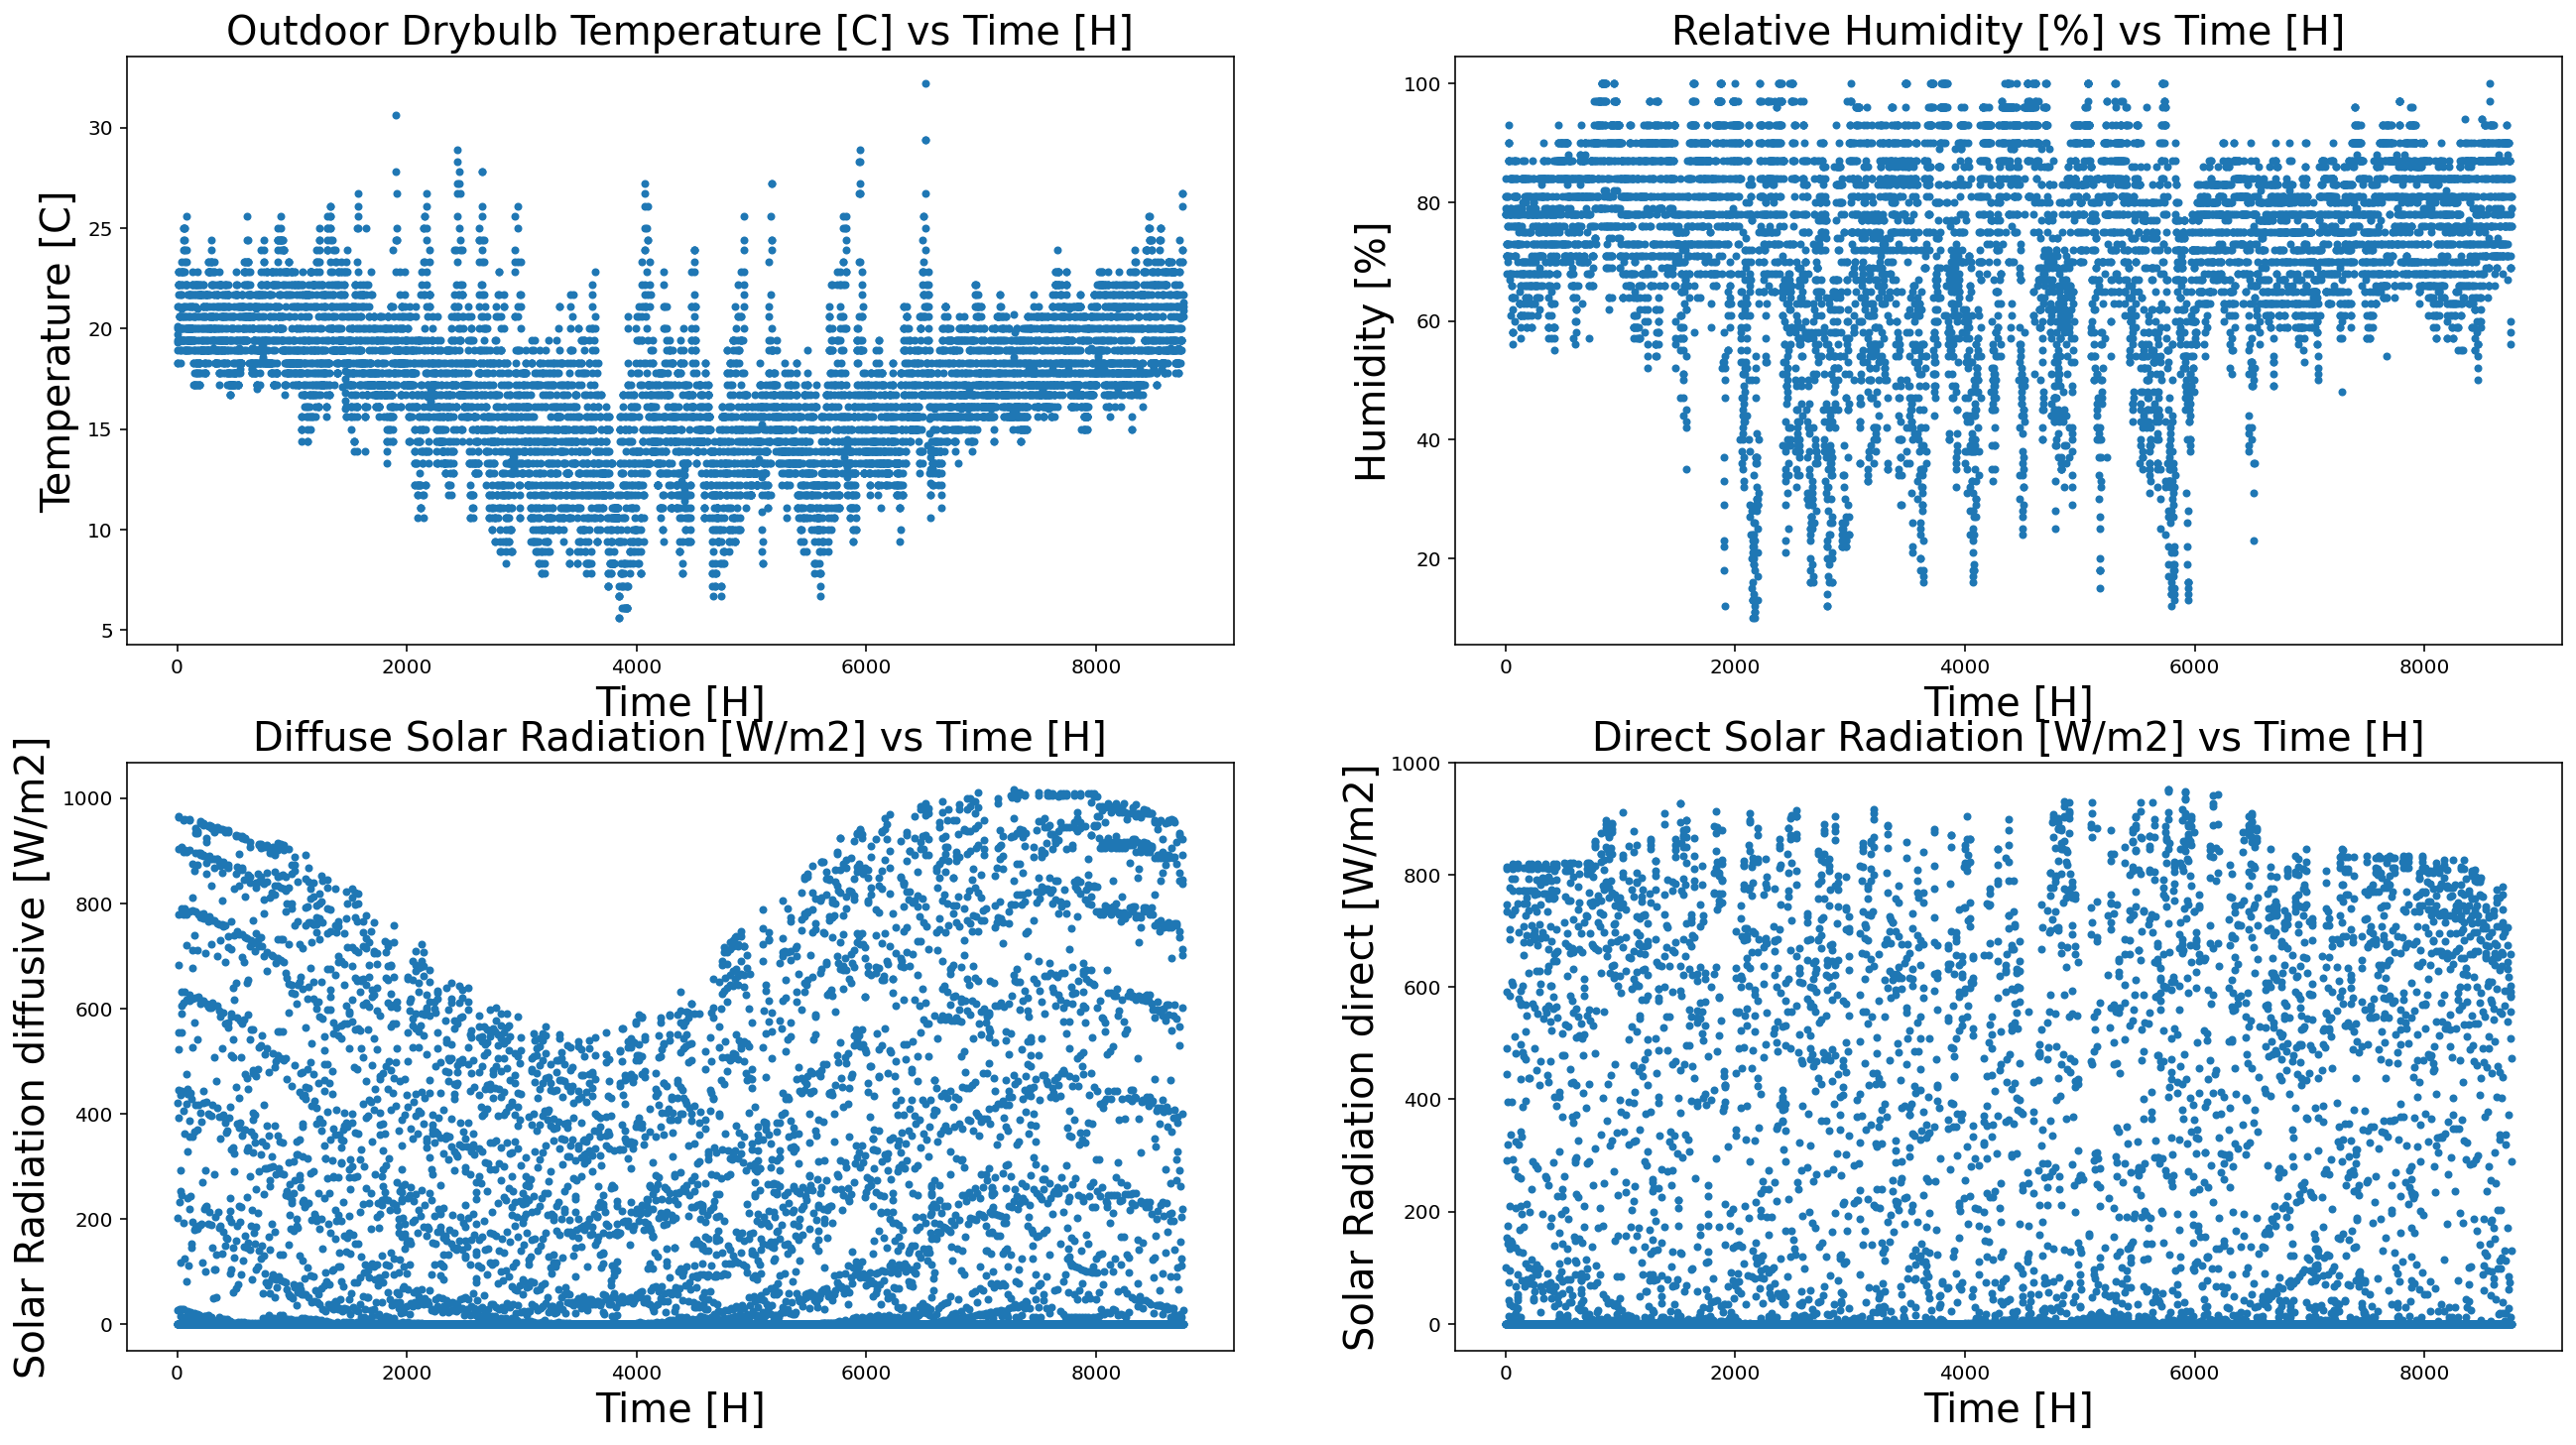
\includegraphics[width = 0.9\textwidth]{weatherData.png}
		  }
		  \par}
		\caption{Weather data.}
		\label{fig:weather}
		\end{figure}
		
		It was not explicitly stated in the data description starting day and hour, however, based on observations of temperature and solar radiation the starting day looks to be around July.
	\item Electricity pricing measured in $\frac{kW}{h}$, which changes dynamically and periodically depending on the hour of the day, type of the day (working day/weekend) and month. 17 Weeks of the year have increased prices due to the current season - winter/summer. The most expensive electricity price occurs between 15:00-19:00 daily. Electricity prices for the same hours are reduced during the weekends by approximately half, see figure~\ref{fig:pricing}.
		
		\begin{figure}[H]
		\centering	
			\subfigure[Whole Year]{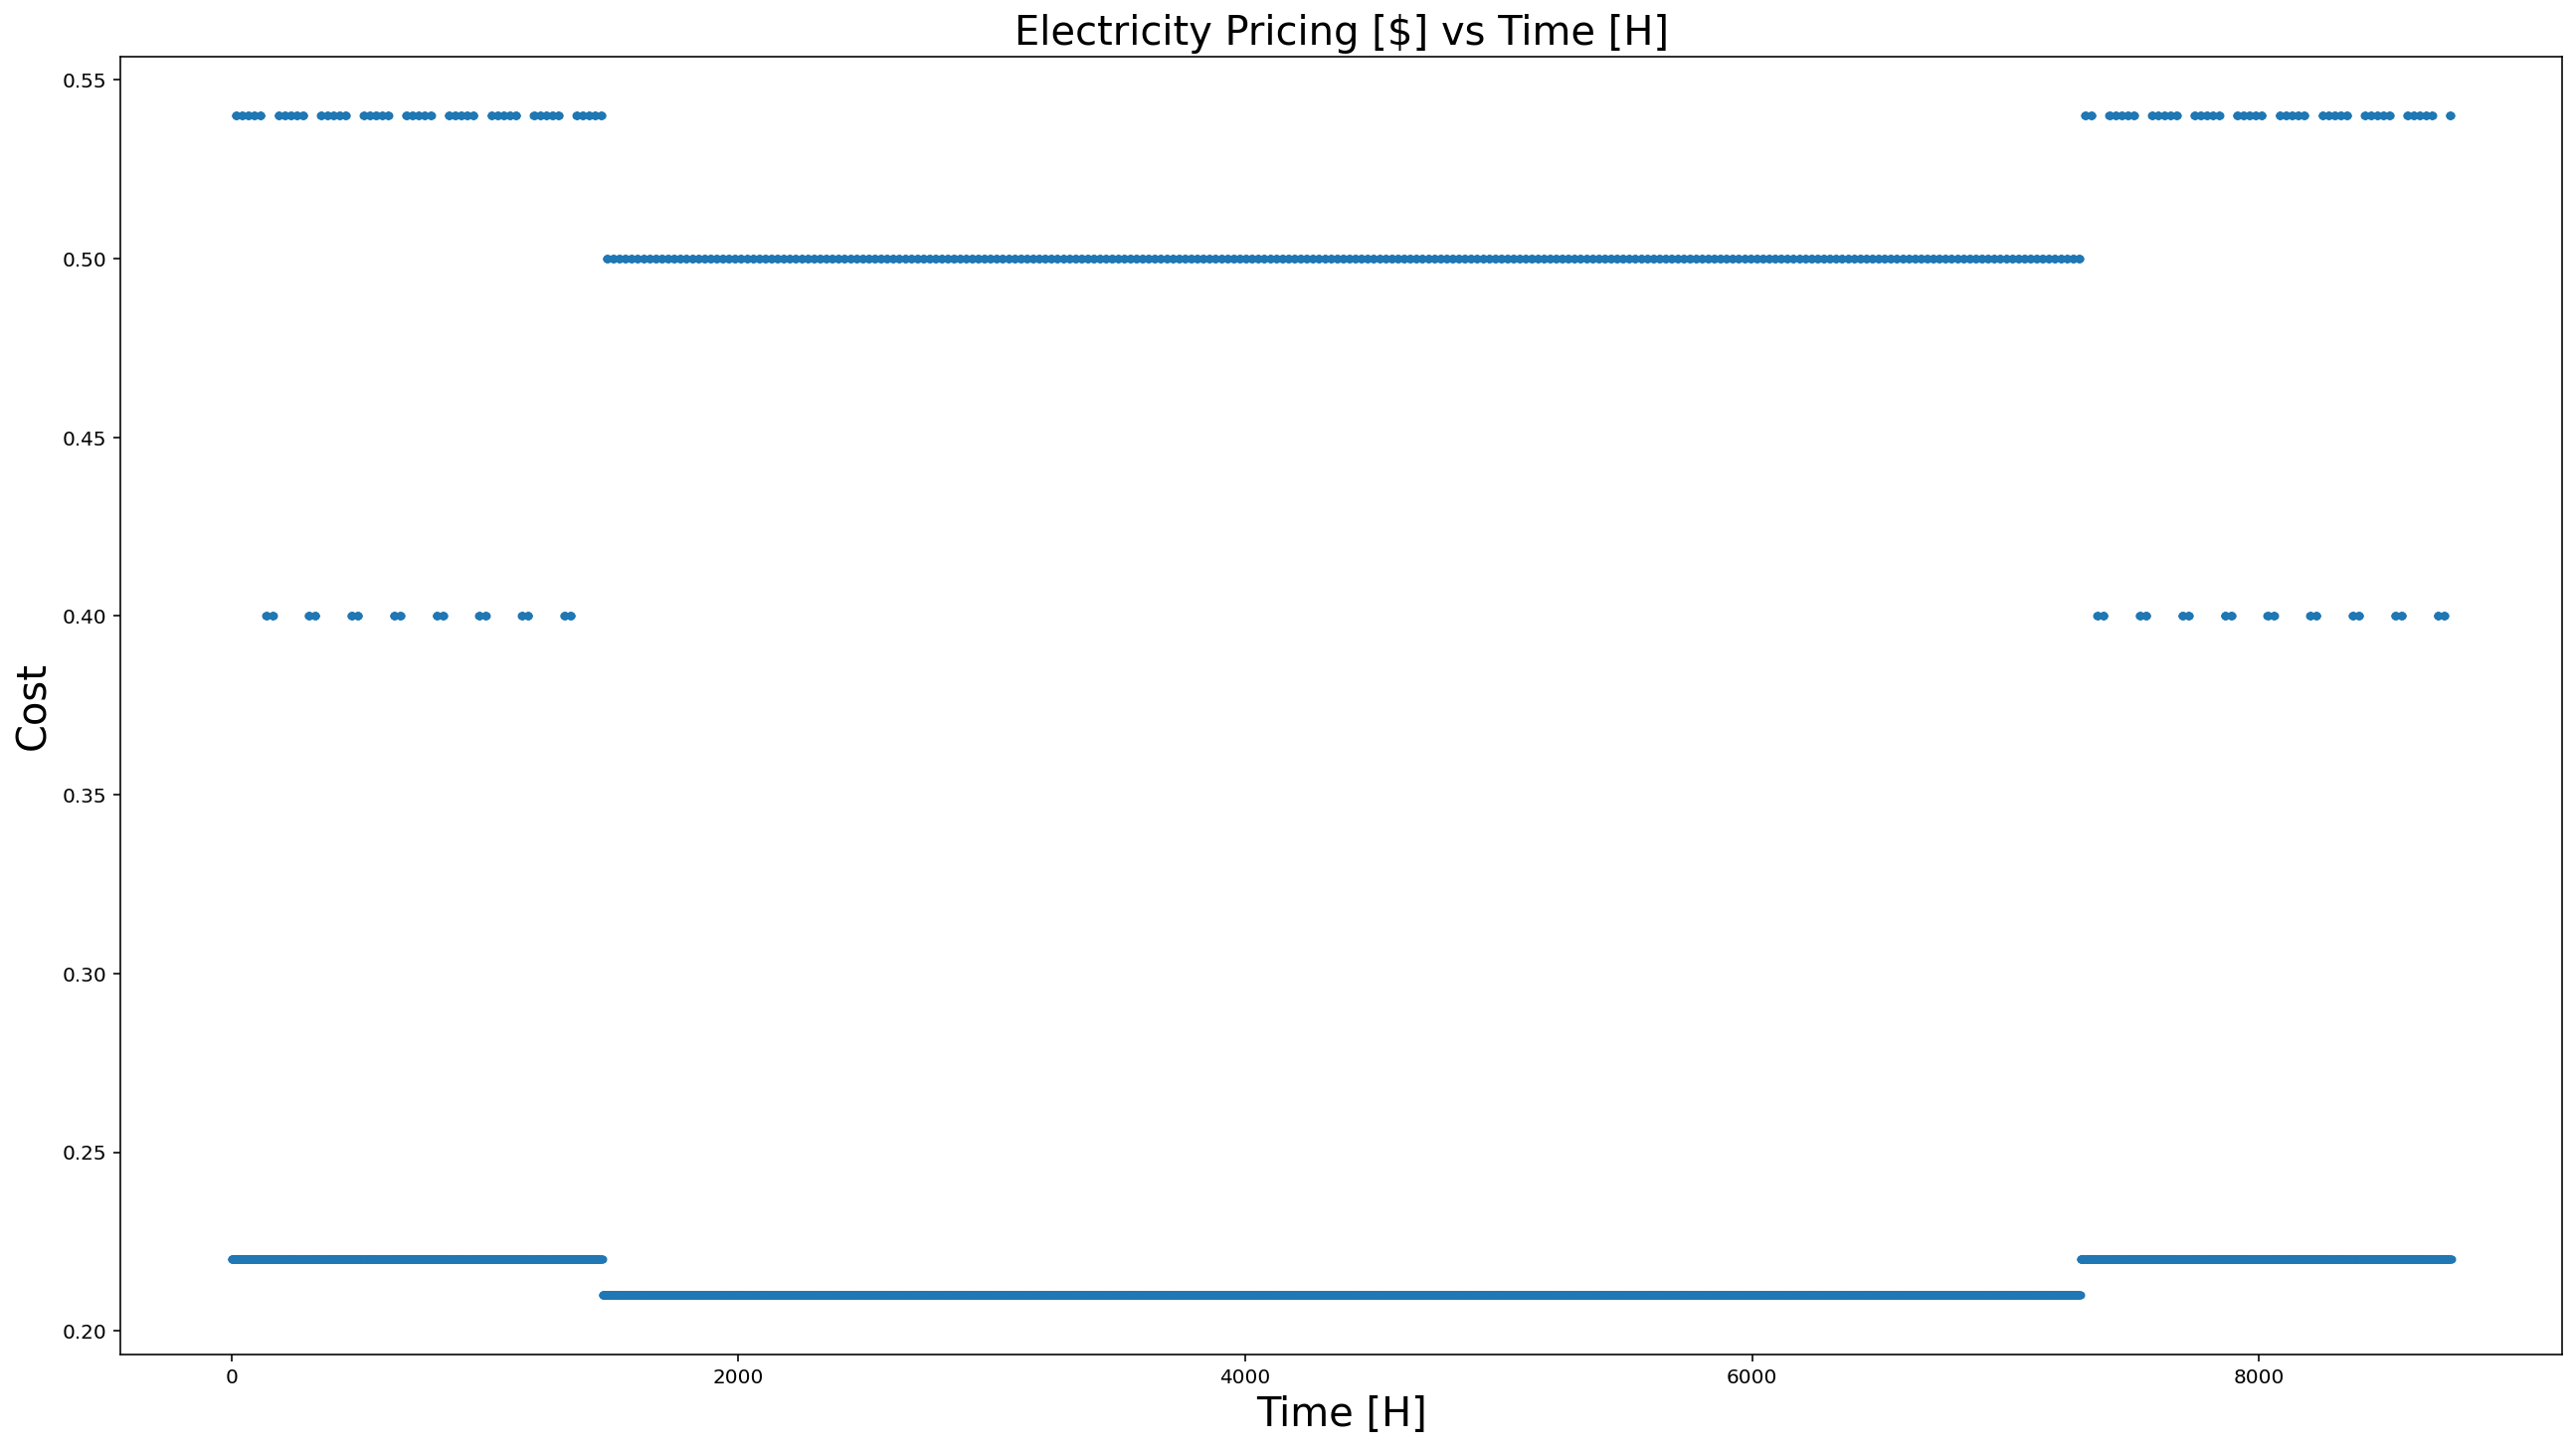
\includegraphics[height=0.25\textwidth]{pricingDataAll.png} \label{fig:Pricing all}} \quad
			\subfigure[Transition weeks]{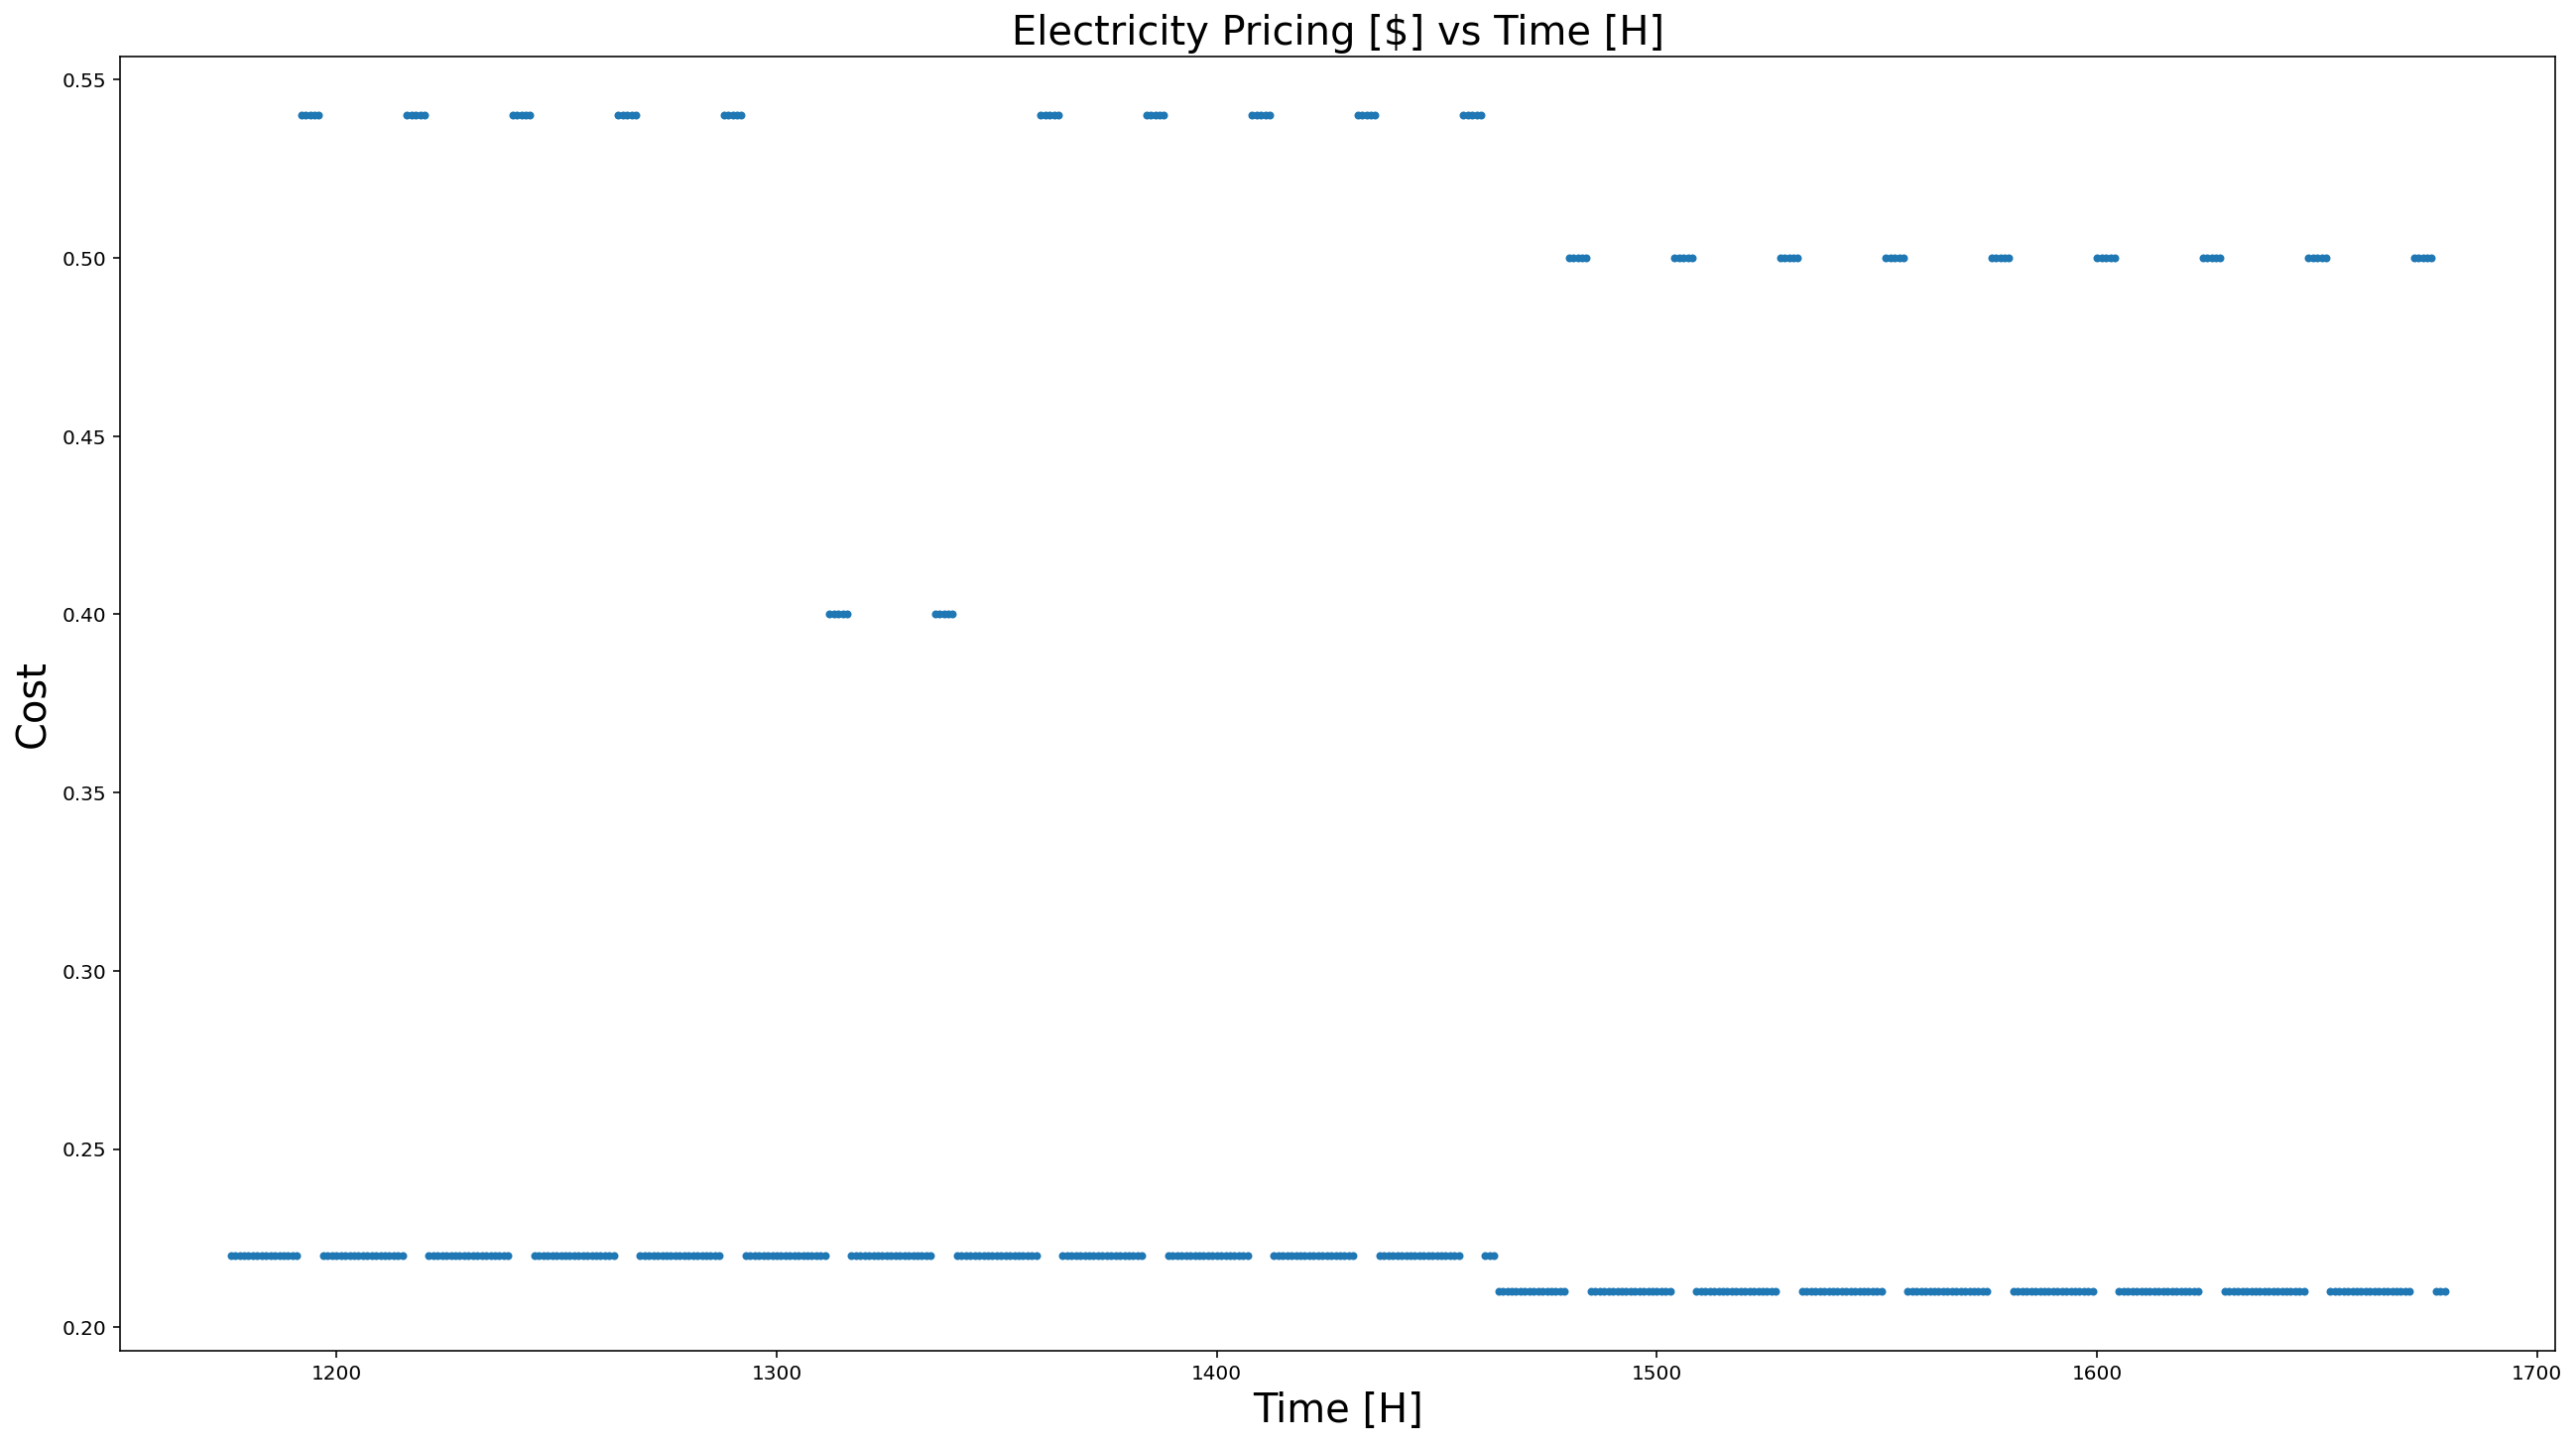
\includegraphics[height=0.25\textwidth]{pricingDataTransition.png} \label{fig:pricing}}
		\caption{\small Electricity pricing.}
		\end{figure}
	\item Carbon intensity (figure~\ref{fig:carbon}), which is the amount of carbon dioxide gas $CO_2$ generated per $\frac{kW}{h}$ on the power plant. Containing a single column measured in $\frac{kg\cdot CO_2}{kW\cdot h}$. 
		\begin{figure}[H]
		{\centering
		  {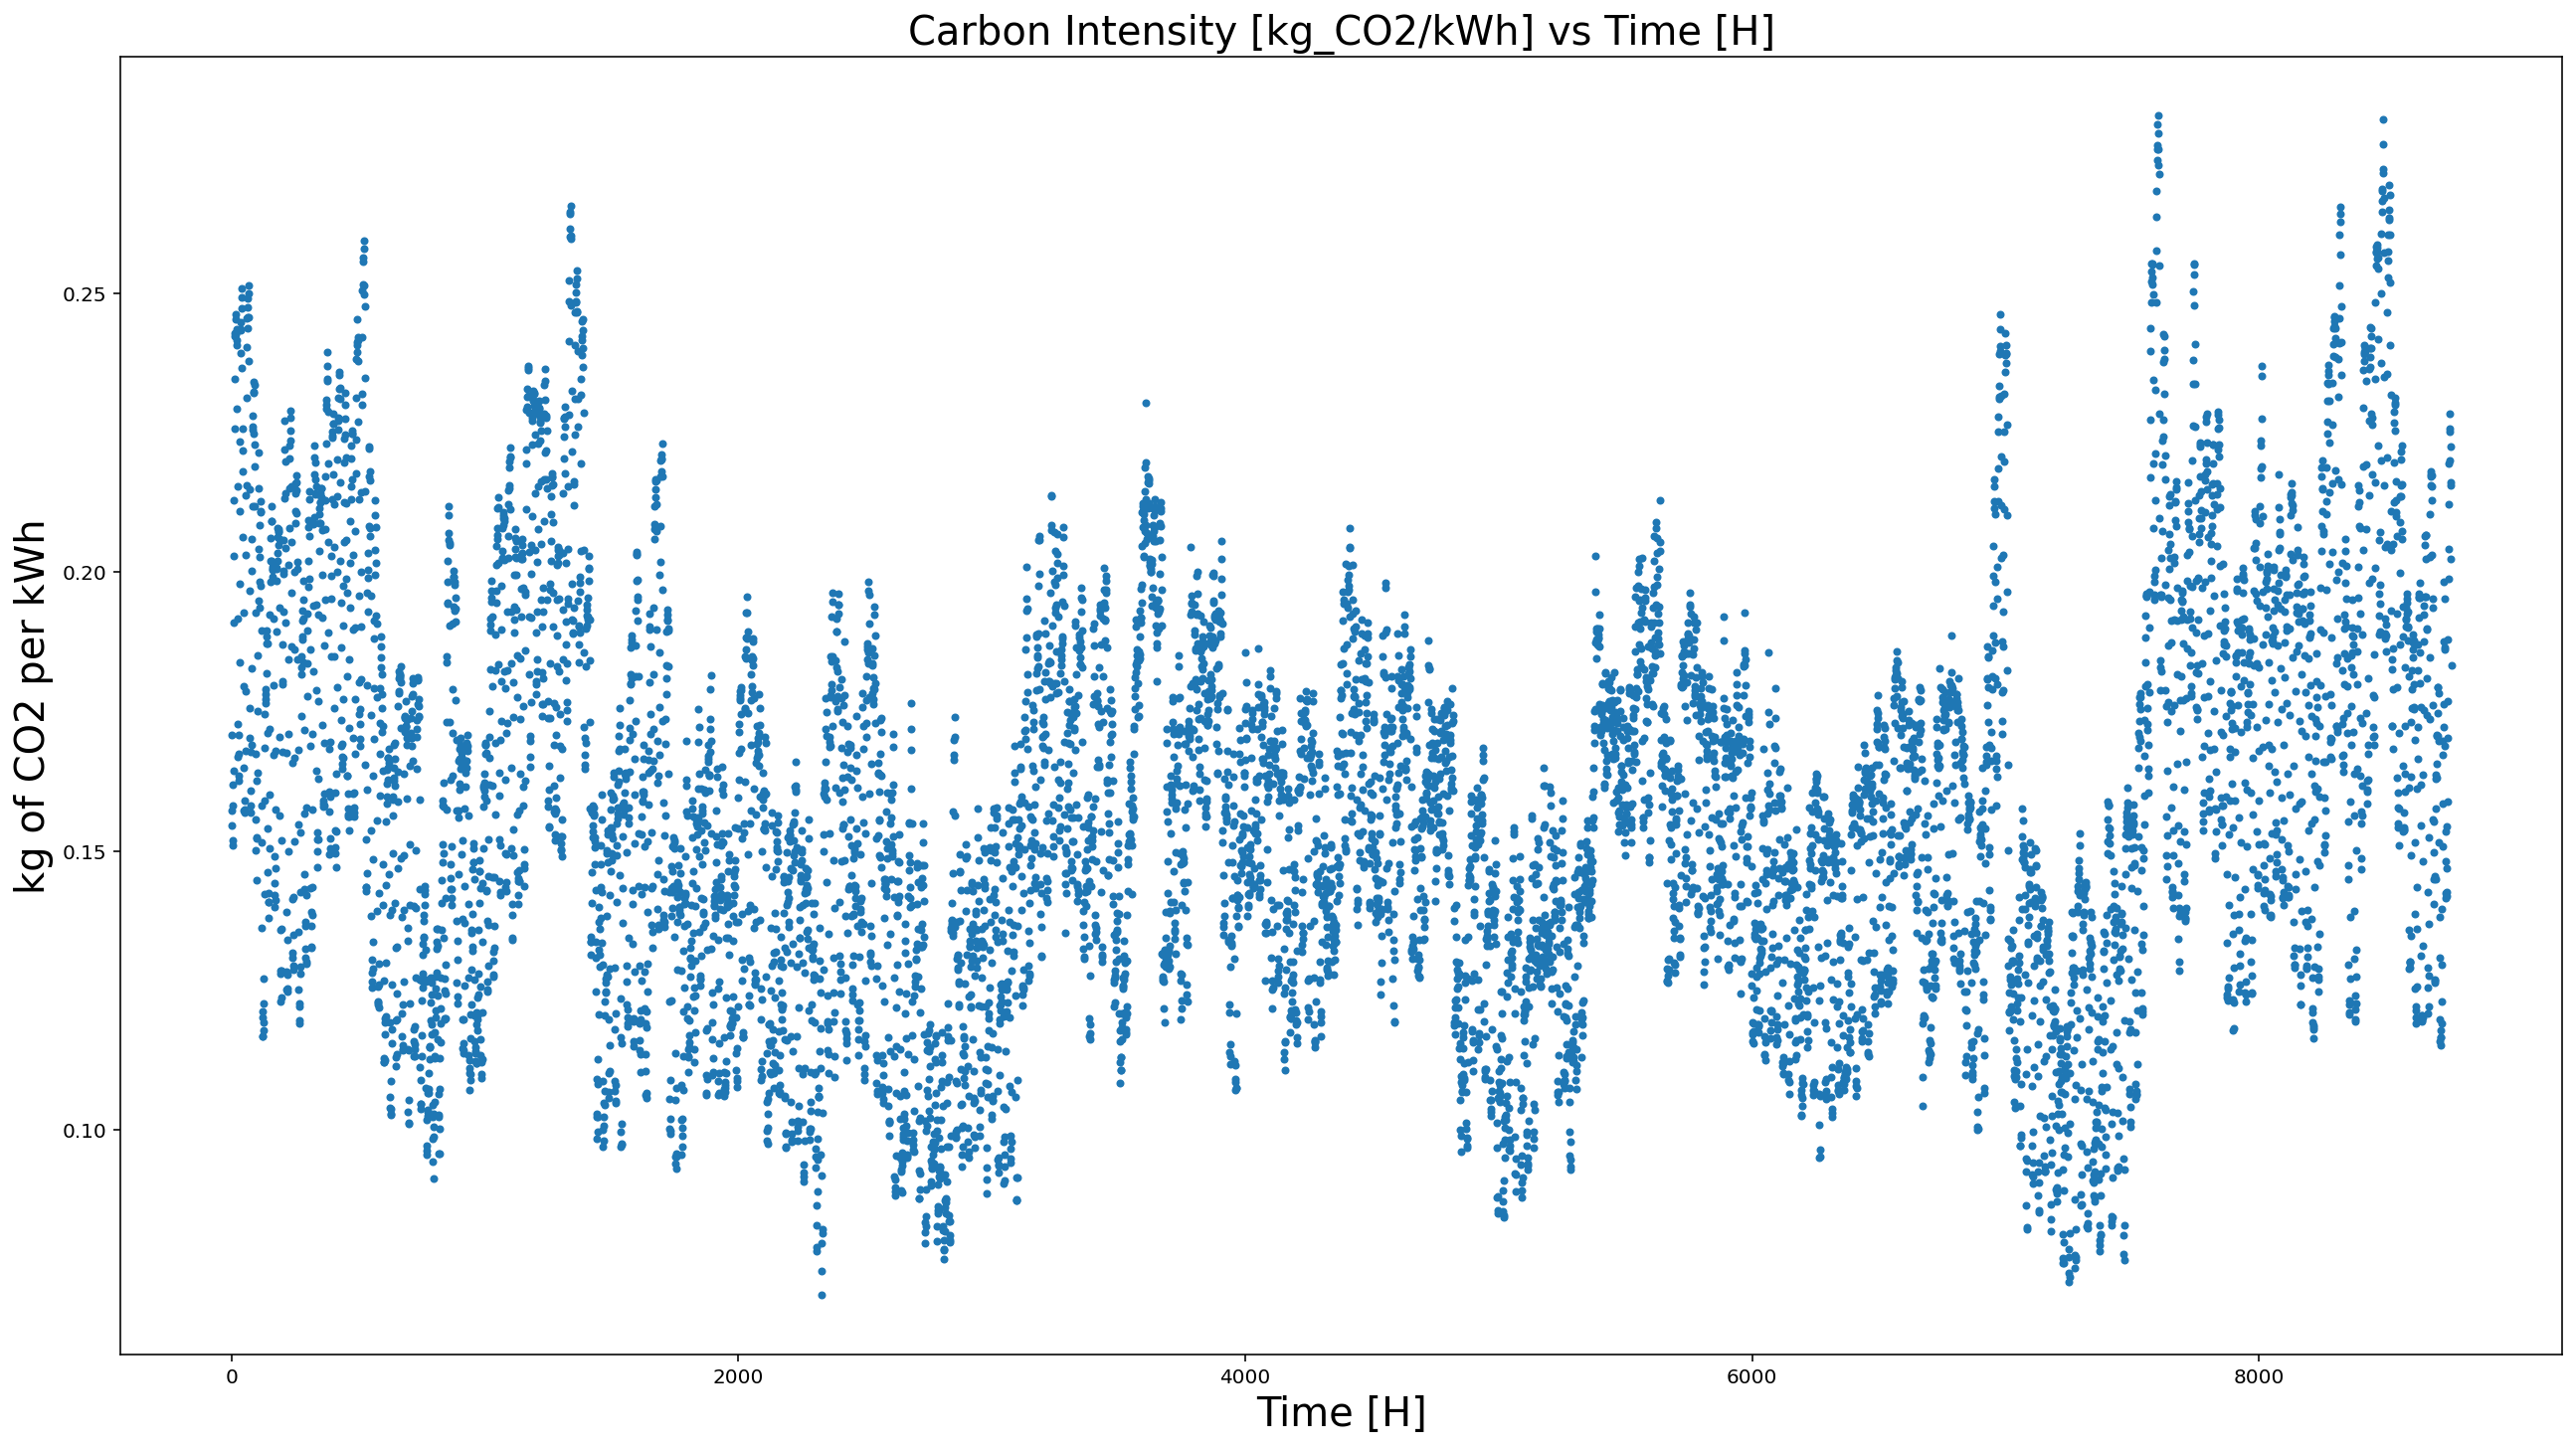
\includegraphics[width = 0.7\textwidth]{carbonIntensity.png}
		  }
		  \par}
		\caption{Carbon intensity data $\frac{kg\cdot CO_2}{kW\cdot h}$.}
		\label{fig:carbon}
		\end{figure}
	\item 

		
	Data for 5 different buildings located in the same neighbourhood of the city, figures~\ref{fig:bd1}-\ref{fig:bdGenCons}. 
		\begin{figure}[H]
		\centering	
			\subfigure[Day type]{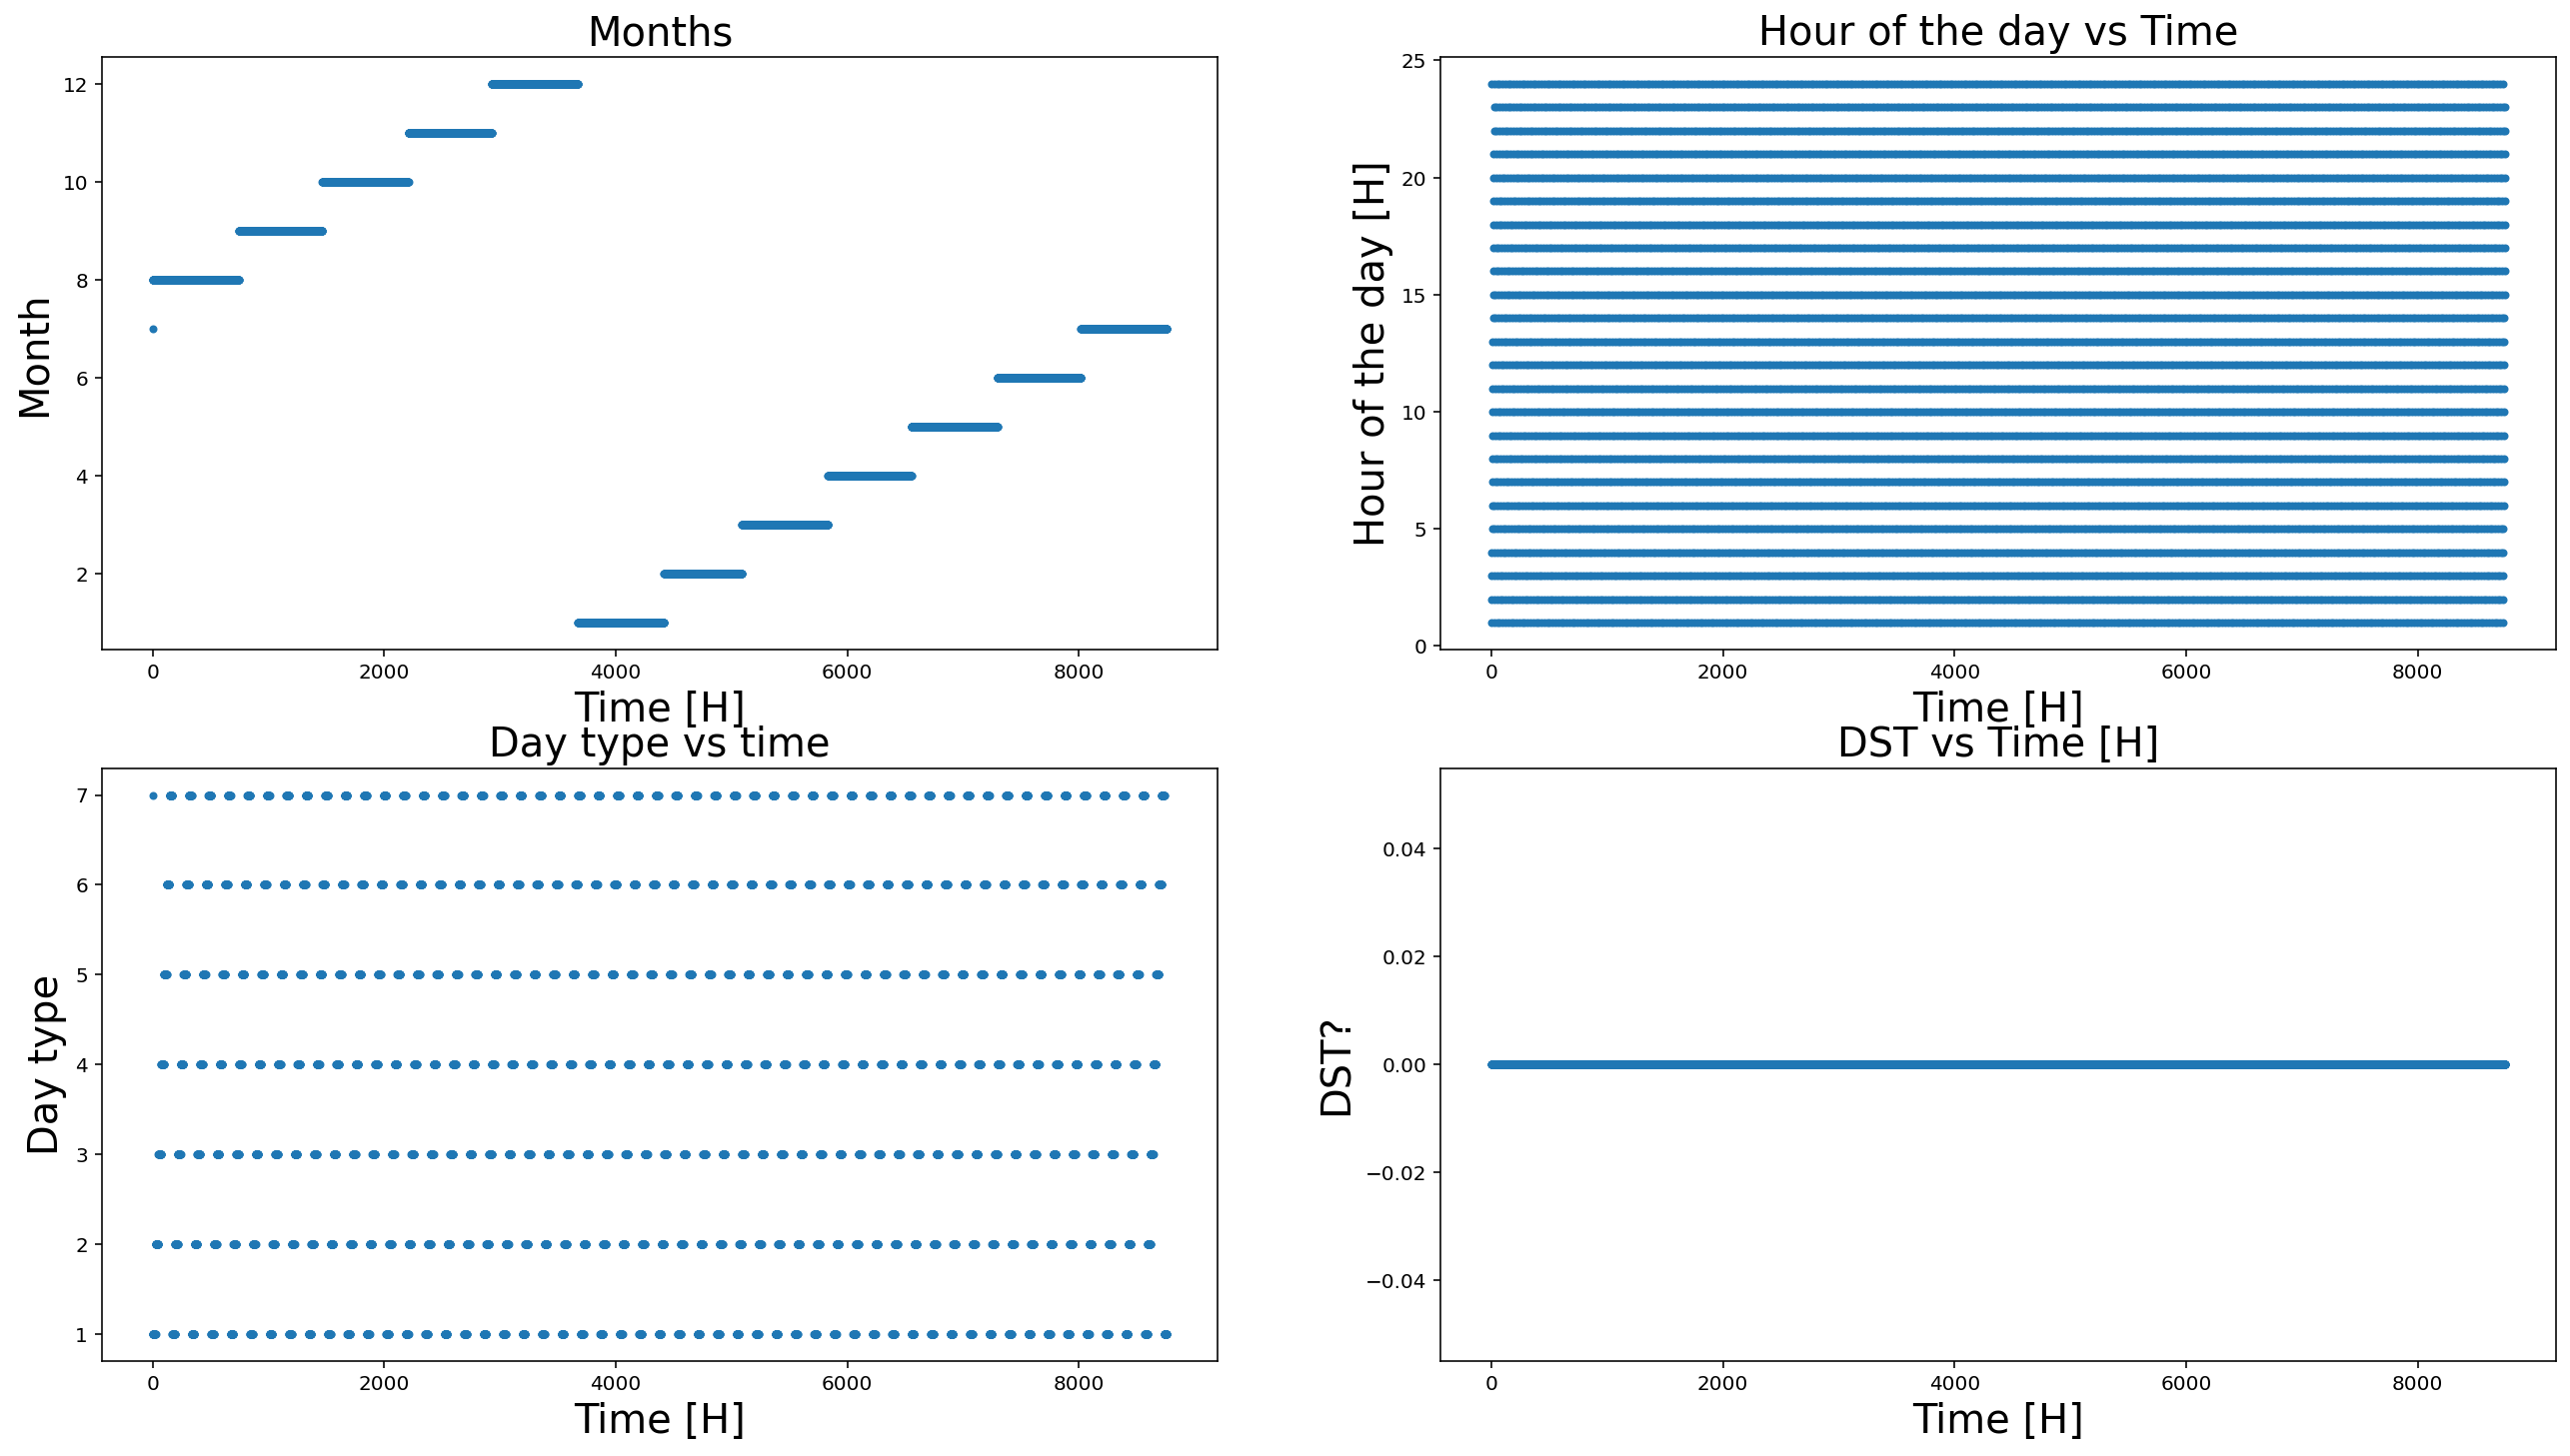
\includegraphics[height=0.25\textwidth]{bd1.png}\label{fig:bd1}} \quad
			\subfigure[Consumption/Generation of electricity by buildings]{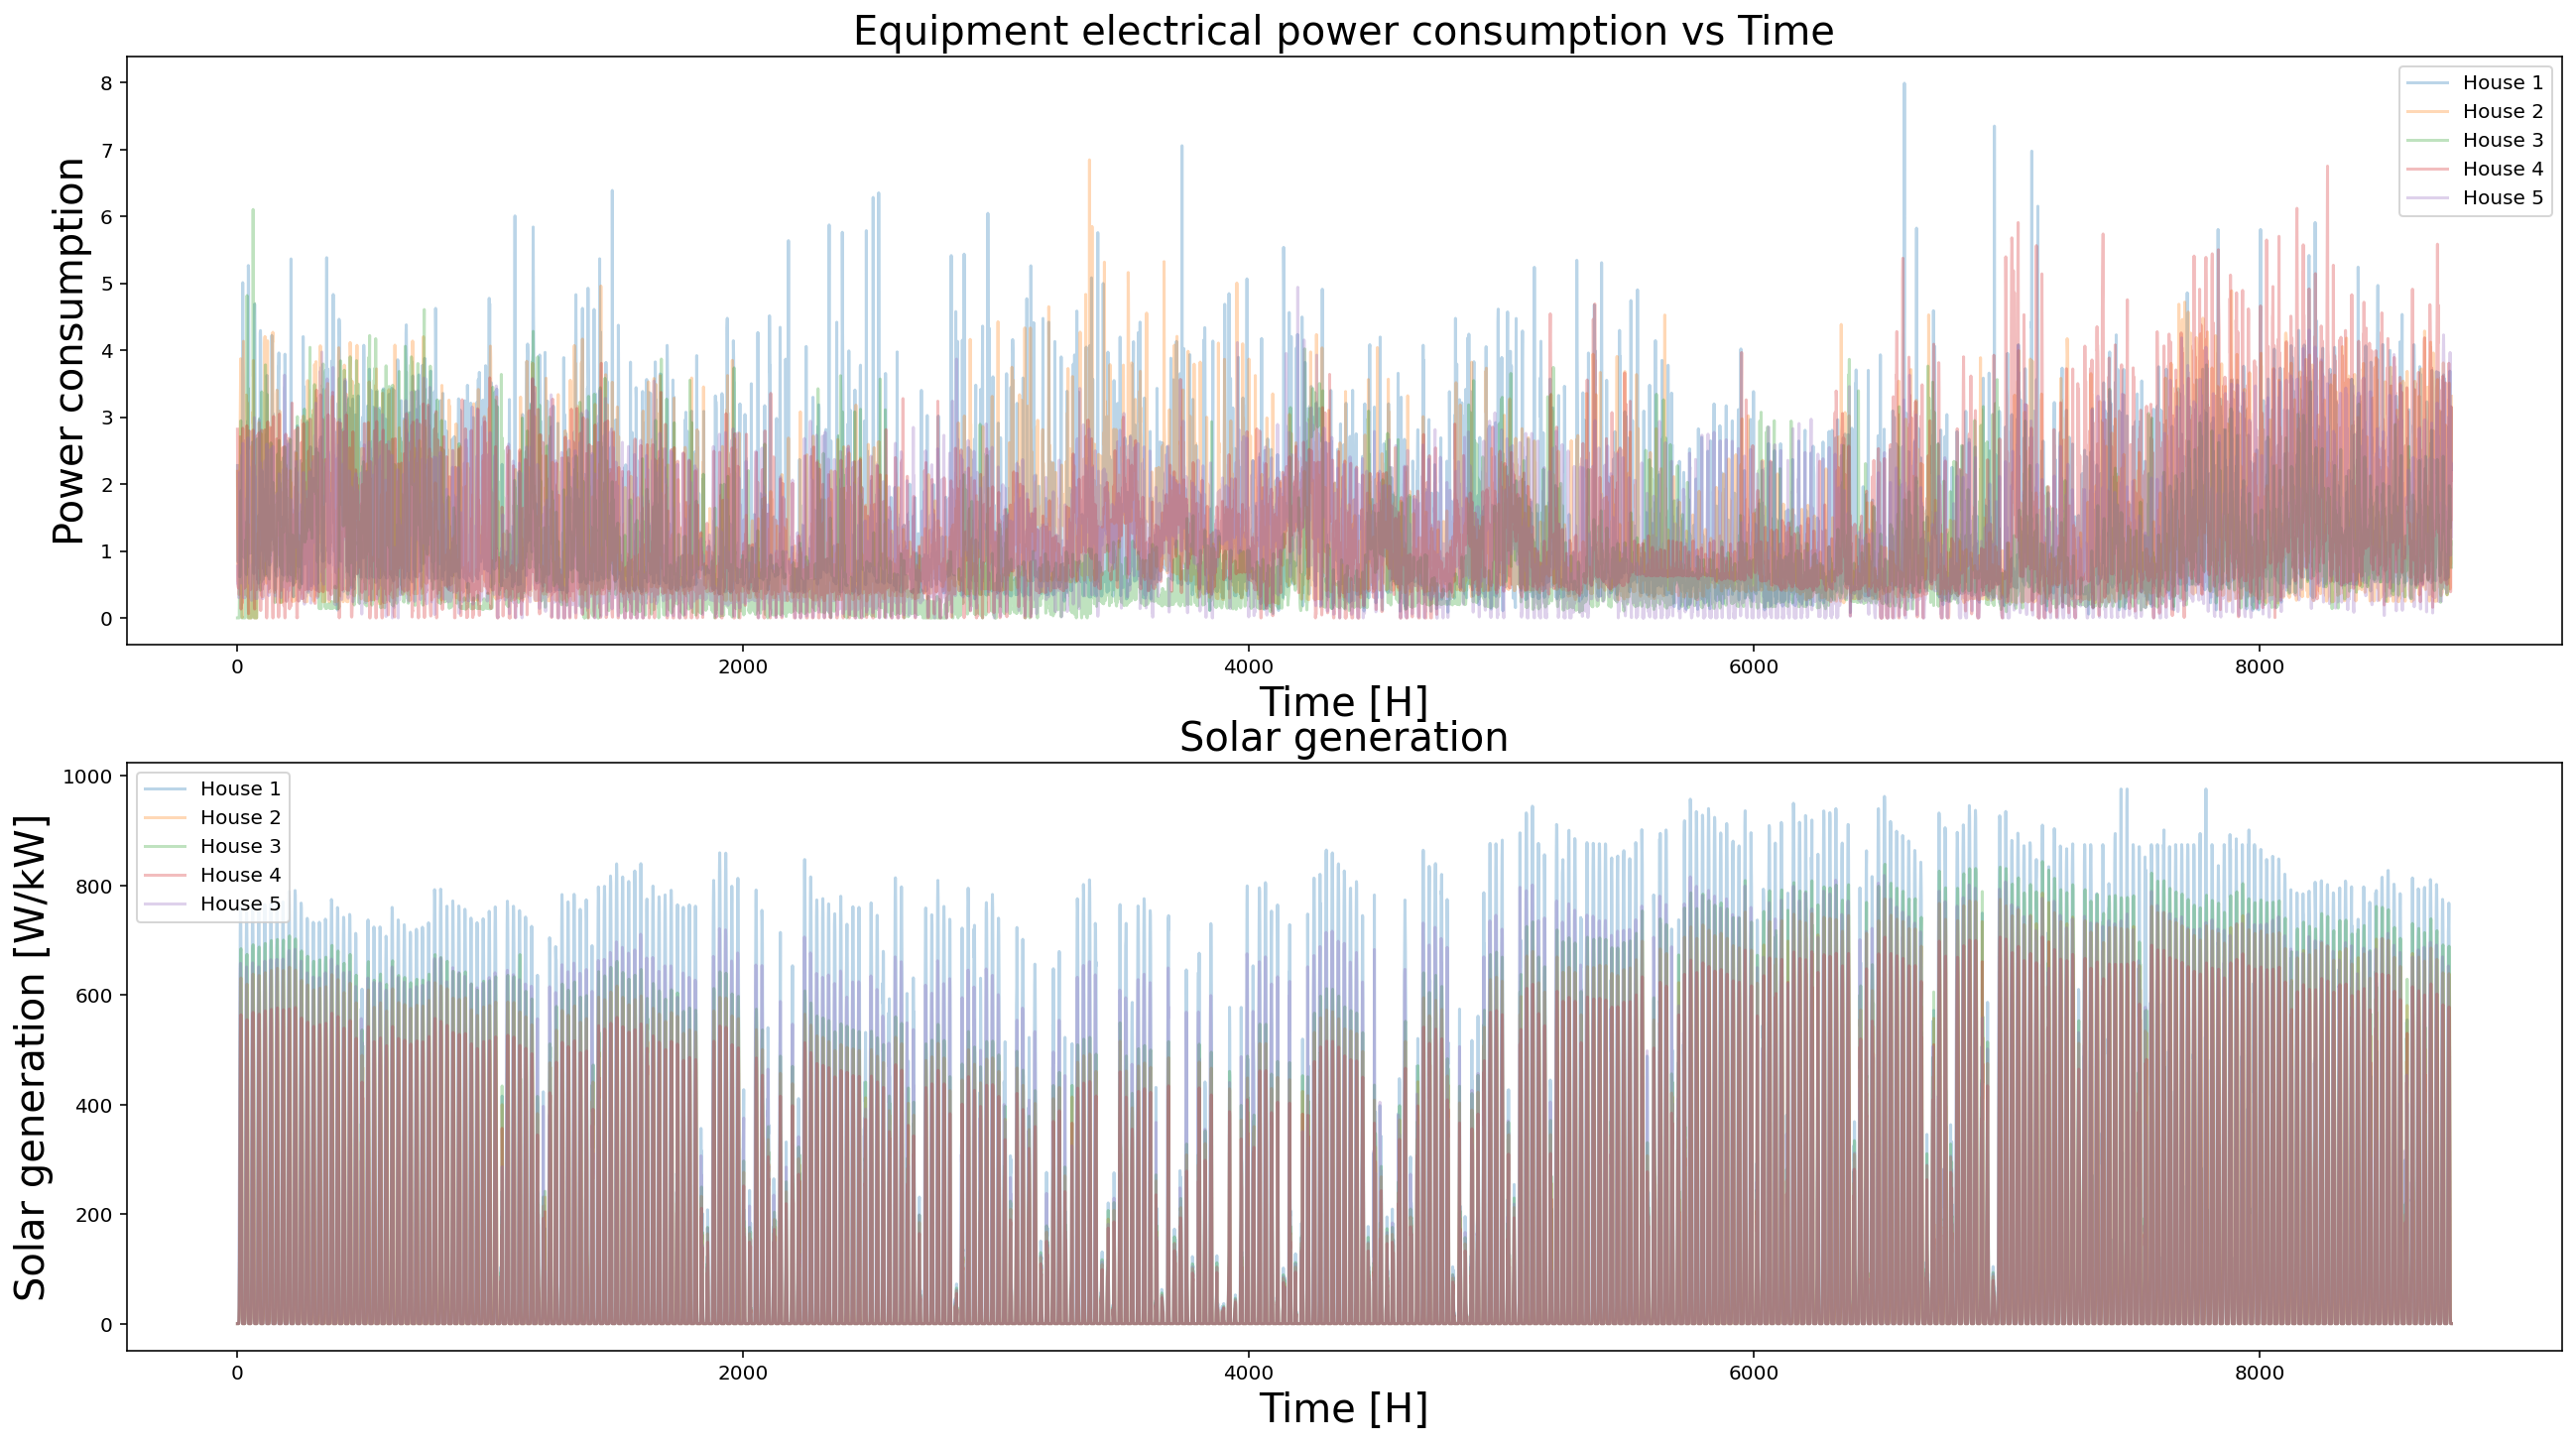
\includegraphics[height=0.35\textwidth]{bdGenCons.png}\label{fig:bdGenCons}}
			\caption{\small Electricity pricing.}
		\end{figure}
		Each building contains:
		\begin{enumerate}
			\item Month	[1-12].
			\item Hour	[1-24].
			\item Day Type	[1-7].
			\item Daylight Savings Status  [0-1]. Changed all to the same time without Daylight Saving [0]. 
			\item Indoor Temperature [C].
			\item Average Unmet Cooling Setpoint Difference [C]	contains no data.
			\item Indoor Relative Humidity [\%]	contains no data.
			\item Equipment Electric Power [kWh].
			\item DHW Heating [kWh].
			\item Cooling Load [kWh].
			\item Heating Load [kWh].
			\item Solar Generation [W/kW].
		\end{enumerate}
		
\end{itemize}

\section{Data augmentation using CTGAN}

As mentioned before, having a limited and small dataset was one of our challenges in this project. In order to tackle this problem we used a data augmentation technique. Data augmentation is a technique to artificially create new data from existing data and significantly increase the diversity of data available for training the models. Most of the models that are used for generating tabular data are based on modelling the probability distribution of rows in the dataset and sampling from the distribution. These models are mainly used for continuous data while our tabular data contains a mix of discrete and continuous columns. One of the frameworks that can be used for generating continuous and discrete data is CTGAN- conditional generative adversarial networks.

CTGAN is a collection of Deep Learning based synthetic data generators for single table data, which are able to learn from real data and generate synthetic data with high fidelity. A GAN consists of two Neural Networks:
\begin{itemize}
	\item A generator that learns to produce fake data;
	\item A discriminator that learns to distinguish the generator’s fake data from the real data.
\end{itemize} 

\begin{figure}[H]
		{\centering
		  {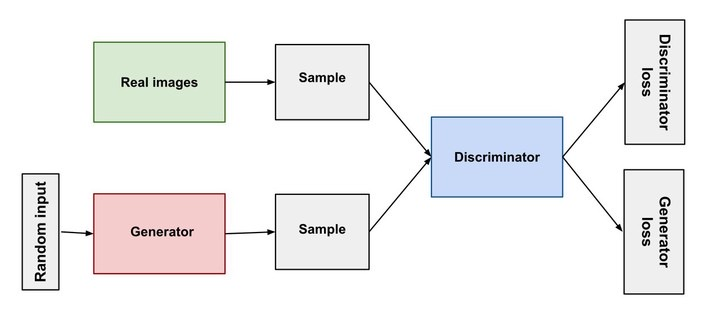
\includegraphics[width = 0.7\textwidth]{CTGAN}
		  }
		  \par}
		\caption{Generating tabular data using GAN.}
		\label{fig:carbon}
		\end{figure}

The two models compete against each other. At the start of the training, the generator is not very good at generating fake data, and the discriminator is able to catch the fake data easily. But as training progresses, the generator learns to get progressively better at generating fake data, and fooling the discriminator, until the discriminator is unable to tell if the input is real or not. This procedure drives the whole system toward optimization.

In this project, we tried to use CTGAN from Synthetic Data Vault (SDV) library to generate and add 1000 rows to our dataset. Although because our data is time series this technique didn't work.

\section{User client and Target Variables}

The dataset provided by the competition is expected to have some score evaluation algorithm, the file \verb!local_evaluation.py! or its modifications. The target values are 
\begin{enumerate}
	\item \verb!Average Price Cost! - reduce electricity consumption from the power plant by individual buildings.
	\item \verb!Average Emmision Cost! - reduce $CO_2$ emissions into the atmosphere by individual buildings.
	\item \verb!Average Grid Cost!. - the rate of the whole district's electricity consumption.
\end{enumerate}








\section{Algorithmic approach}

The Simplest rule-based client (RBC) was based on releasing the stored energy during the day hours of 9 AM to 9 PM if any excess is generated since battery capacity is limited. Whereas during evening and nighttime 10 PM to 8 AM, we are also able to store DHW and/or cooling energy. The performance looked not so promising. 

\begin{verbatim}
	user@user citylearn-2022-starter-kit-master % python3 local_evaluation.py 
	Starting local evaluation
	Num Steps: 1000, Num episodes: 0
	Num Steps: 2000, Num episodes: 0
	Num Steps: 3000, Num episodes: 0
	Num Steps: 4000, Num episodes: 0
	Num Steps: 5000, Num episodes: 0
	Num Steps: 6000, Num episodes: 0
	Num Steps: 7000, Num episodes: 0
	Num Steps: 8000, Num episodes: 0
	Episode complete: 1 | 
	Latest episode metrics: 
	{'price_cost': 1.0696759094682255, 
	'emmision_cost': 1.1792710334714276, 
	'grid_cost': 1.0748389680788613}
	=========================Completed=========================
	Average Price Cost: 1.0696759094682255
	Average Emmision Cost: 1.1792710334714276
	Average Grid Cost: 1.0748389680788613
	Total time taken by agent: 1.1828435109600832s
	user@user citylearn-2022-starter-kit-master % 
\end{verbatim}


\section{Reinforcement learning approach}

Reinforcement learning is an important type of machine learning where an agent learns how to behave in the environment by performing actions and seeing results \cite{freecodecamp}.

In recent years, we have seen many advances in this exciting area of ​​research. For example, DeepMind and Deep Q Learning Architecture in 2014, defeating the Go champion with AlphaGo in 2016, and OpenAI and PPO in 2017, among others.

Tasks to address prior choosing models/algorithms:
\begin{itemize}
	\item What is reinforcement learning and why rewards are central?
	\item Three approaches to reinforcement learning.
	\item What does "deep" mean in deep reinforcement learning?
\end{itemize}

It is very important to master these aspects before diving into the implementation of reinforcement learning agents. The idea behind reinforcement learning is that an agent will learn from the environment by interacting with it and getting rewards for performing actions.

Learning through interaction with the environment comes from our natural experience. Imagine a child in the living room. The child sees a fireplace and approaches it. Nearby is warm, and it feels good - positive reward +1. The child understands that fire is a positive thing. But then the kid tries to touch the fire. It burns his hand - negative reward -1. The child has just realized that fire is positive when it is at a sufficient distance since fire produces heat. But if the child gets close to it, it will get burned. This is how people learn through interaction. Reinforcement learning is simply a computational approach to learning through actions.

As an example, let's say an agent is learning to perform some task. Reinforcement Learning (RL) can be modelled as a loop \cite{sutton2018reinforcement} that works like this

\begin{figure}[H]
	{\centering
	  {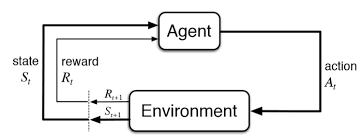
\includegraphics[width = 0.5\textwidth]{rlDiagram}
	  }
	  \par}
	\caption{Sample diagram of RL approach.}
	\label{fig:rl-diagram}
\end{figure}

\begin{itemize}
	\item The agent receives state $S_t$ from the environment. 
	\item Based on this state $S_t$, the agent takes action $A_t$.
	\item Environment moves to new state $S_{t+1}$.
	\item Environment gives some reward to $R_{t+1}$.
\end{itemize}


This RL cycle produces a sequence of states, actions, and rewards.
The agent's goal is to maximize the expected cumulative reward.

\subsection{The central idea of ​​the Reward Hypothesis}\textbf{}

Why is the agent's goal to maximize the expected cumulative reward? Well, reinforcement learning is based on the idea of ​​the reward hypothesis. All goals can be described by maximizing the expected cumulative reward.

Therefore, in reinforcement learning, to achieve the best behaviour, we need to maximize the expected cumulative reward.

The cumulative reward at each time step t can be written as:

\begin{equation}
	\begin{gathered}
	G_t=R_{t+1}+R_{t+2}+\ldots, \\
	\text{which is equivalent to:}\\
	G_t=\sum_{k=0}^T R_{t+k+1}
	\end{gathered}
\end{equation}


However, in reality, one cannot simply add such rewards. Rewards that arrive earlier (early in the game) are more likely because they are more predictable than rewards later in the game. To reduce the reward, we do the following:
\begin{enumerate}
	\item Determine the discount rate, called the $\gamma$ (gamma). It must be between 0 and 1.
	\item The larger the gamma, the smaller the discount. This means that the learning agent is more concerned with long-term rewards.
	\item On the other hand, the smaller the gamma, the greater the discount. This means that short-term rewards are in priority.
\end{enumerate}

Accumulated working reward, taking into account discounting, is as follows:

\begin{equation}
\begin{aligned}
G_t= & \sum_{k=0}^{\infty} \gamma^k R_{t+k+1} \text { where } \gamma \in[0,1) \\
& R_{t+1}+\gamma R_{t+2}+\gamma^2 R_{t+3 \cdots}
\end{aligned}
\end{equation}

Roughly speaking, each reward will be scaled down by gamma to time. As time step increases, a future reward becomes less and less likely.

\subsection{Episodic or continuous tasks}

A task is an instance of a reinforcement learning problem. We can have two types of tasks:

\begin{enumerate}
	\item \textbf{Episodic task}. In this case, we have a start point and an end point (terminal state). This creates an episode: a list of states, actions, rewards, and new states.
	\item \textbf{Continuous Tasks}. These are tasks that go on forever (no terminal state). In this case, the agent must learn to choose the best actions and interact with the environment at the same time.

		For example, an agent that performs automated stock trading. There is no start point and no end state for this task. The agent continues to run until we decide to stop it.
\end{enumerate}

\subsection{Monte Carlo Method vs Time Difference Method}

There are two ways to learn:
\begin{itemize}
	\item Collect the rewards at the end of an episode and then calculate the maximum expected future reward - the Monte Carlo approach.
	\item Estimate the reward at each step - time difference.
\end{itemize}

\textbf{Monte Carlo}

When the episode ends - the agent reaches a "terminal state", then the agent looks at the total accumulated reward to see how well it did. In the Monte Carlo approach, the reward is received only at the end of the complete episode.

Then user starts a new episode with added knowledge. The agent makes better decisions with each iteration.

\begin{equation}
V\left(S_t\right) \leftarrow V\left(S_t\right)+\alpha\left[G_t-{V\left(S_t\right)}\right],
\end{equation}
where $\alpha$ is the learning rate.


Running more and more episodes, the agent will learn to perform better and better.

\textbf{Time Differences: Learning at Each Time Step}

The Temporal Difference Learning (TD) method will not wait until the end of the episode to update the maximum possible reward. It will update $V(S_t)$ depending on the experience gained.

This method is called TD(0) or incremental TD (updates the utility function after any single step).


\begin{equation}
	V\left(S_t\right) \leftarrow V\left(S_t\right)+\alpha\left[R_{t+1}+\gamma V\left(S_{t+1}\right)-V\left(S_t\right)\right],
\end{equation}
where discounted value on the next step $\gamma V(S_{t+1})$ is added to the discounted cumulative reward.

TD methods only wait for the next time step to update values. At the time $t+1$, a TD target is formed using the reward $R_{t+1}$ and the current score $V(S_{t+1})$.

The TD goal is an estimate of what is expected by effectively updating the previous estimate $V(S_t)$ to the goal within one step.

\subsection{Three Approaches to Reinforcement Learning}

Now that the main elements of reinforcement learning were identified, we shall move on to three approaches \cite{sutton2018reinforcement} to solving reinforcement learning problems:
\begin{enumerate}
	\item \textbf{Value Based}.
		In such RL, the goal is to optimize the utility function $V(S)$.
		The utility function is a function that tells us the maximum expected reward the agent will receive in each state.
		
		The value of each state is the total amount of reward that the agent can expect to accumulate in the future, starting from that state.

		\begin{equation}
			v_\pi(s)=\mathbb{E}_\pi\left[R_{t+1}+\gamma R_{t+2}+\gamma^2 R_{t+3}+\ldots \mid S_t=s\right],
		\end{equation}
		where $\mathbb{E}_\pi$ is expected of rewards discounted sum $\sum_{i=1}^{\infty}\gamma^iR_{t+{i-1}}$ given state $S_t=s$
		
		The agent will use this utility function to decide which state to select at each step. The agent selects the state with the highest value.
	\item \textbf{Policy based}. In this RL approach, the user wants to directly optimize the policy function $\pi(s)$ without using a utility function. A policy is what determines the behaviour of an agent at a given time 
		
		\begin{equation}
			a = \pi(s),
		\end{equation}		
		where $a$ is an action, $\pi(s)$ is policy(state).
		
		We are studying the function of politics. This allows us to map each state to the best corresponding action.
		
		There are two types of policy:
\begin{itemize}
	\item \textbf{Deterministic}: A policy in a given state will always return the same action.
	\item \textbf{Stochastic}: Displays the probability of distribution over actions, namely
		\begin{equation} 
			\pi(a \mid s)=\mathbb{P}\left[A_t=a \mid S_t=s\right],
		\end{equation}
		meaning that policy $\pi$ of performing an action $a$ given state $s$ is a probability of taking a particular action $A_t=a$ conditioned to a state $S_t=s$. The policy directly indicates the best action for each step.
\end{itemize}
		
	\item \textbf{Model Based}. In this RL approach, the user models the environment. This means that the user creates a model of the behaviour of the environment. The problem is that each environment will need a different view of the model. 
\end{enumerate}

\subsection{Deep Reinforcement Learning}


Deep Reinforcement Learning introduces deep neural networks to solve reinforcement learning problems – hence the name “deep”. This approach is completely avoided and stated just as acknowledgement.



\section{Addressing the problem with Soft Actor-Critic (SAC) approach}

%\subsection{Soft Actor-Critic (SAC) approach}

\begin{figure}[H]
	{\centering
	  {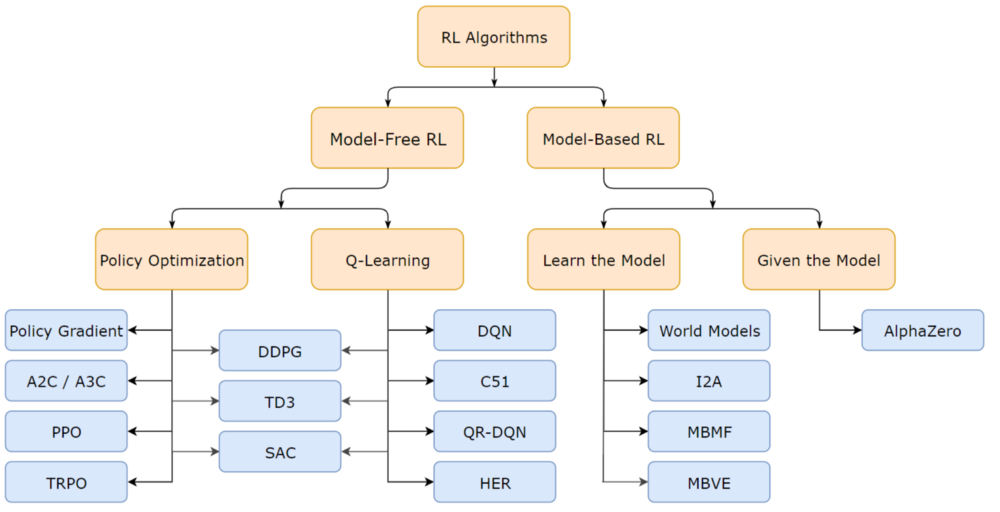
\includegraphics[width = \textwidth]{rlHierarchy}
	  }
	  \par}
	\caption{Hierarchy of RL algorithms.}
	\label{fig:rl-hierarchy}
\end{figure}


A few algorithms and their combinations were recommended in the readme data file. For the purpose of the current project, SAC was chosen arbitrarily since estimated setup and computation time could barely be estimated. 

Figure~\ref{fig:rl-hierarchy} represents a diagram of the relationship between the existing families of reinforcement learning algorithms. As seen
from the hierarchy, the policy optimization family is the most extensive. It is also the most commonly used and most effective in most cases. SAC is a combination of Policy based and Value-based approaches and is model free. 

The main feature of SAC is entropy regularization. The action policy is designed in such a way that the trade-off between expected reward and entropy, which is a measure of randomness in the action policy, is optimized. This trade-off is closely related to the relationship between efficiency and research within the policy of action. The higher the entropy, the more possible new options are considered in the learning process. Entropy control can also help avoid a "local optimum" situation.

To fully describe how SAC works, it is necessary to describe exactly how reinforcement learning occurs under conditions where there is control over entropy.

Entropy is a variable that determines how random another random variable can be. So, the higher the entropy, the less biased the random variable is.

%% 
The data was cut into episodes lasting one week each starting on Sunday midnight and ending on Saturday 23:59. The split led to a total of 5 datasets of ~52 episodes each. Optimization was performed only on two parameters - \verb!price_cost! and \verb!emission_cost! (\verb!grid_cost! was omitted) since a single episode ran even over two variables takes approximately an hour on a modern laptop/computer (see figure~\ref{fig:ep-mem-use}~ from Weights and Biases team run data\cite{wandb}). 

\begin{figure}[H]
	{\centering
	  \subfigure{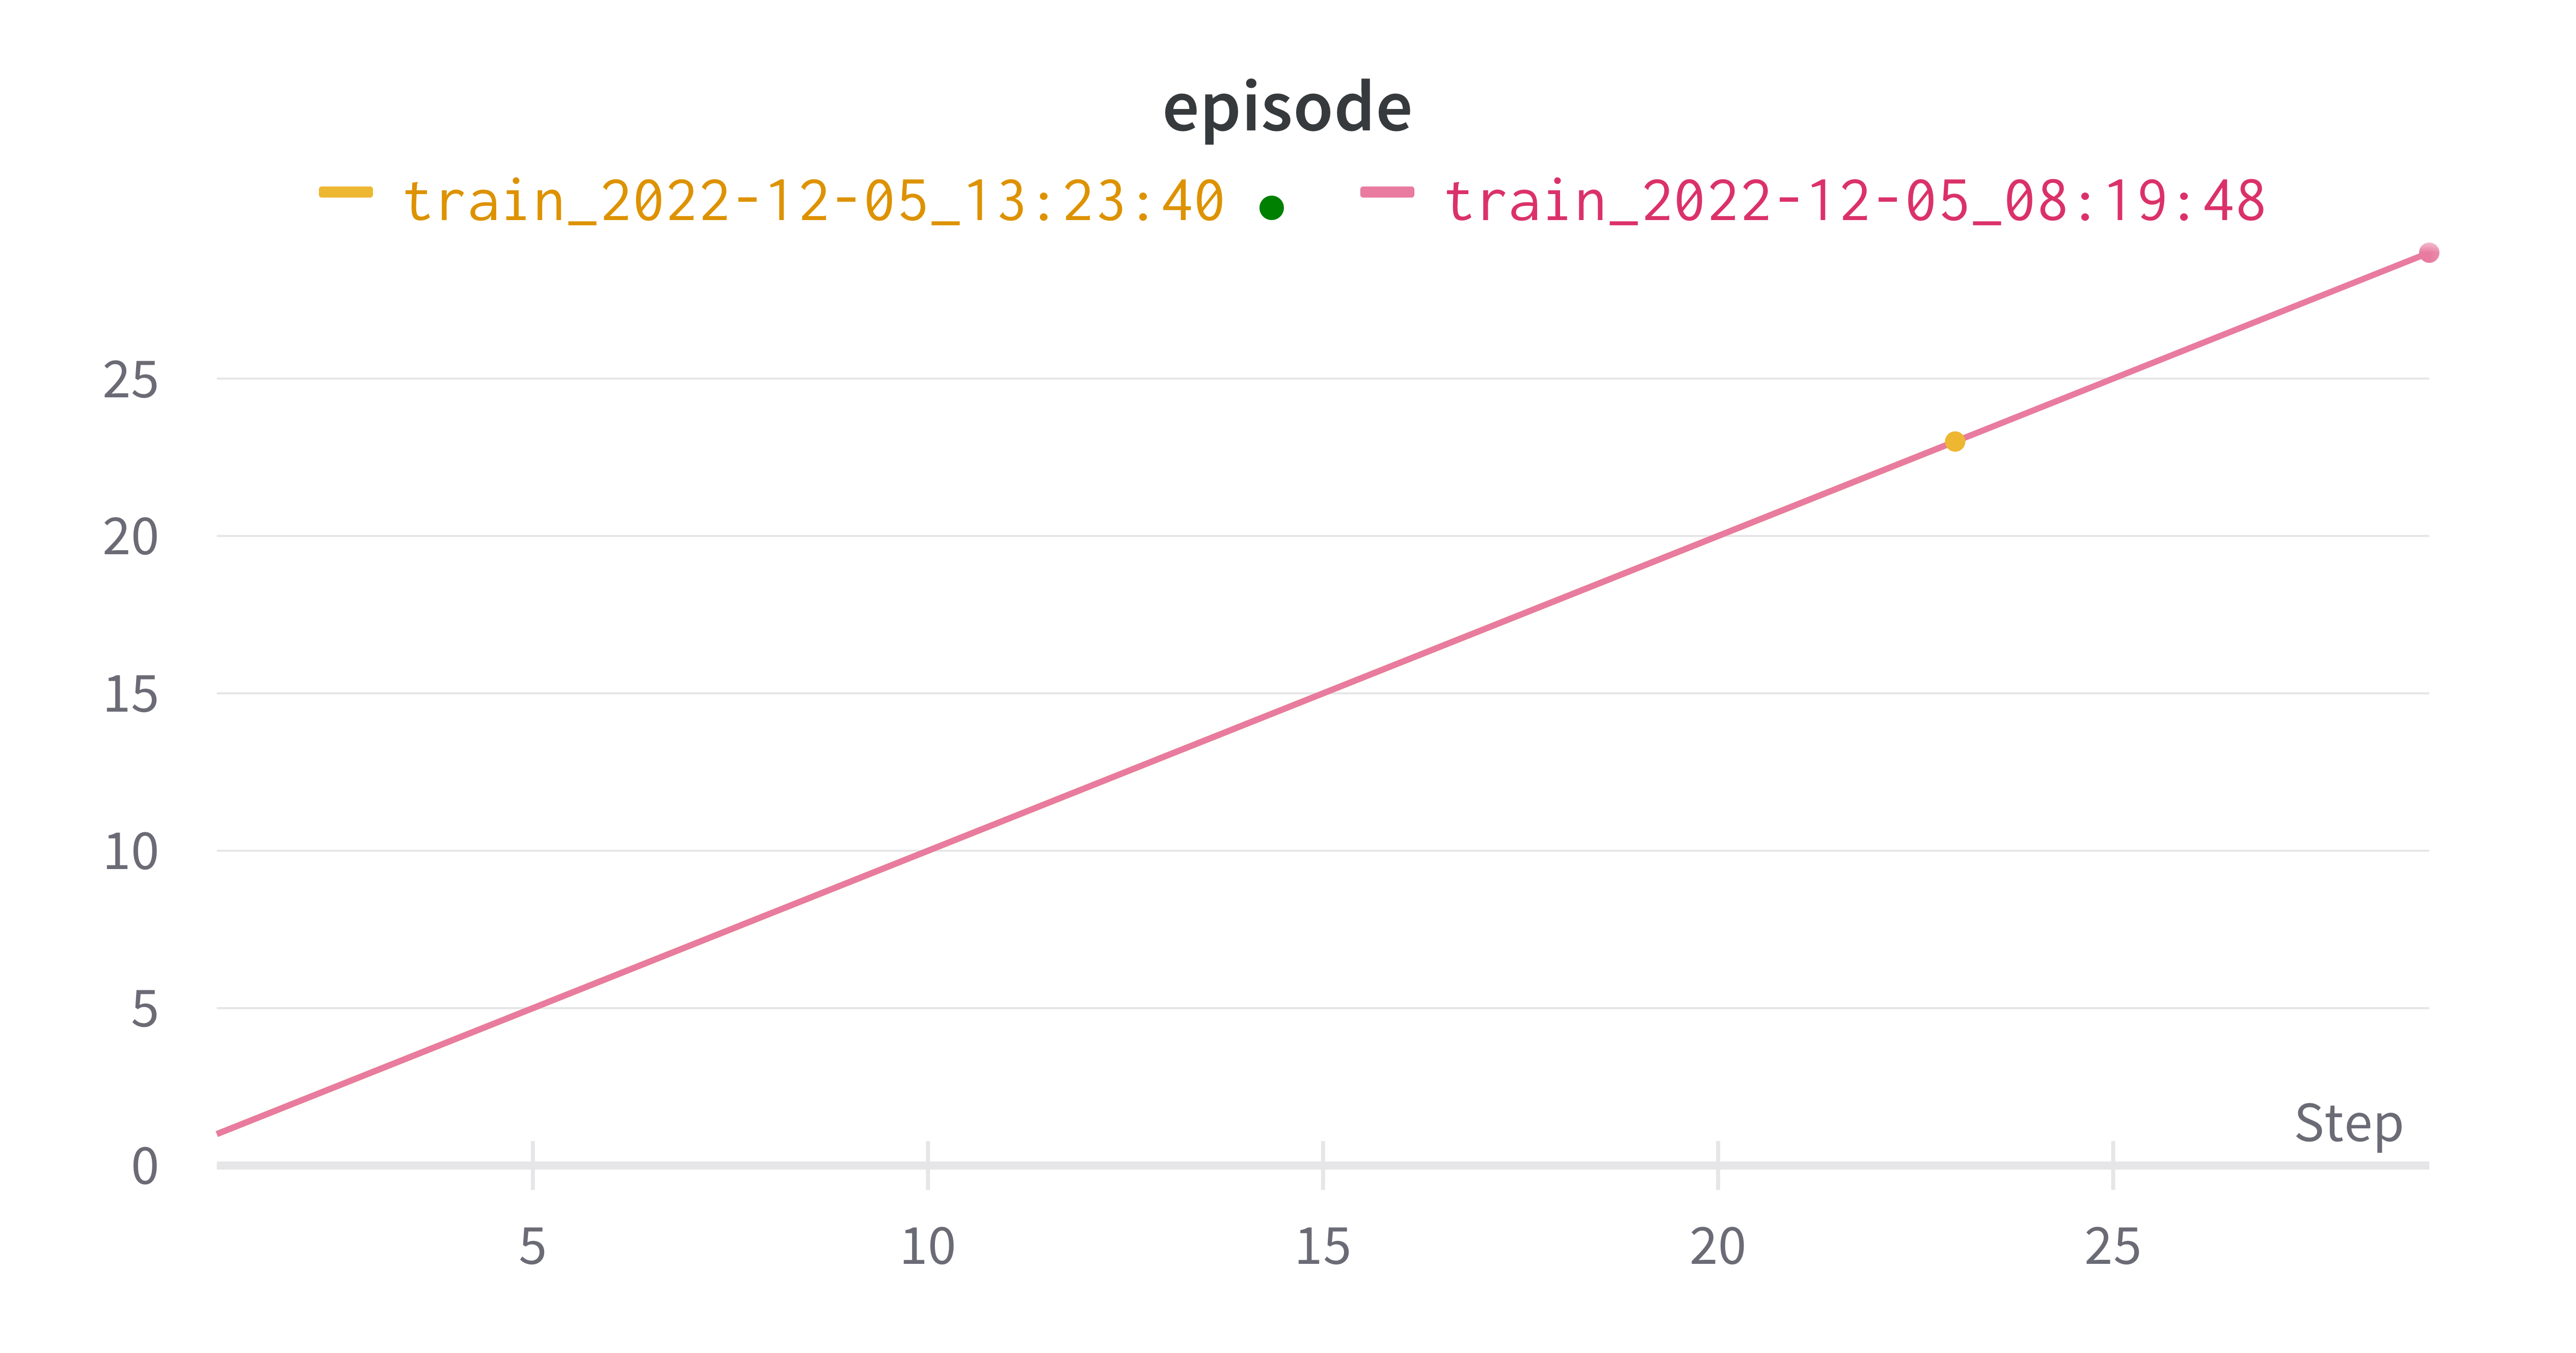
\includegraphics[width = 0.5\textwidth]{episodes}
	  \subfigure{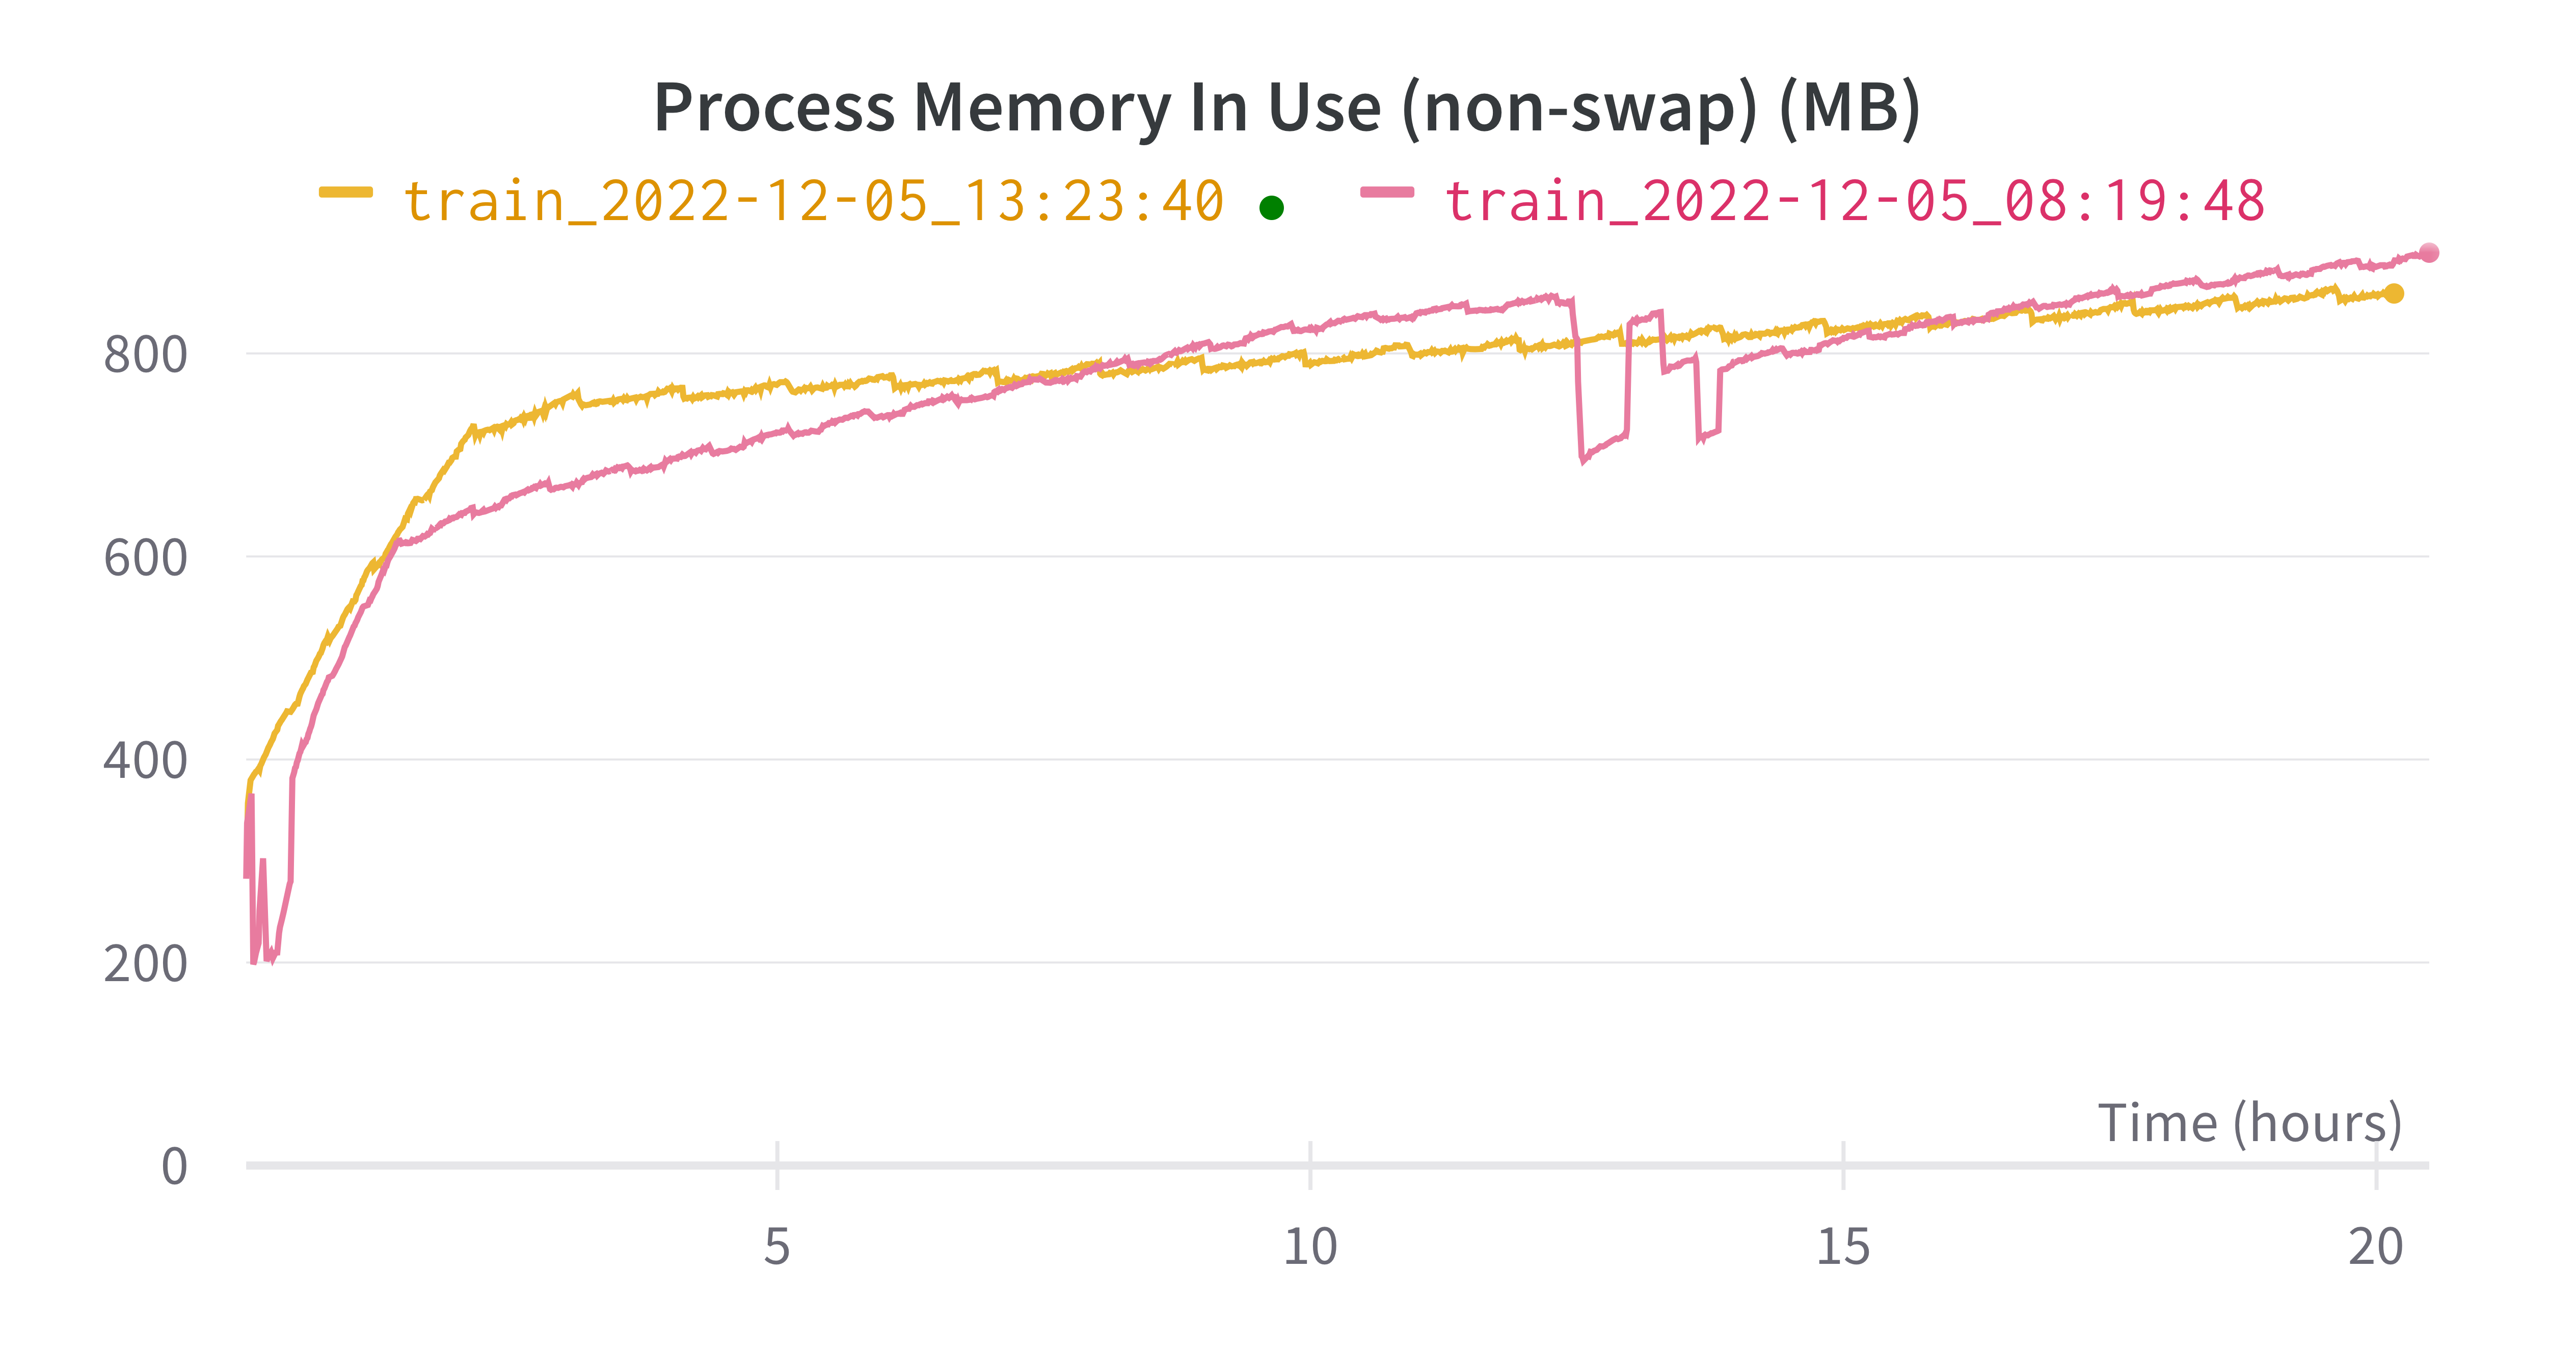
\includegraphics[width = 0.5\textwidth]{memoryUse}}
	  }
	  \par}
	\caption{Episodes and Process memory usage - Laptop (pink) and Desktop(orange).}
	\label{fig:ep-mem-use}
\end{figure}

Due to the behaviour of time (hour/day/month) in the dataset being periodic, i.e. midnight and 1 AM, Sunday and Saturday, December and January are close a normalization was applied. Resulting in periodic functions with values between 0 and 1.

A \verb!wandb! - Weights \& Biases extension was used to keep track of the runs and generate plots of results. The algorithm used \verb!NumPy, torch, gym! and other libraries.

With a help of the Computer Science department\cite{gitlab}, the algorithm was run on a Compute Canada cluster on Graphical Processing Units (GPU) using Compute Unified Device Architecture (CUDA). 



\section{Results and conclusions}
	
	\begin{figure}[H]
		\centering	
			\subfigure{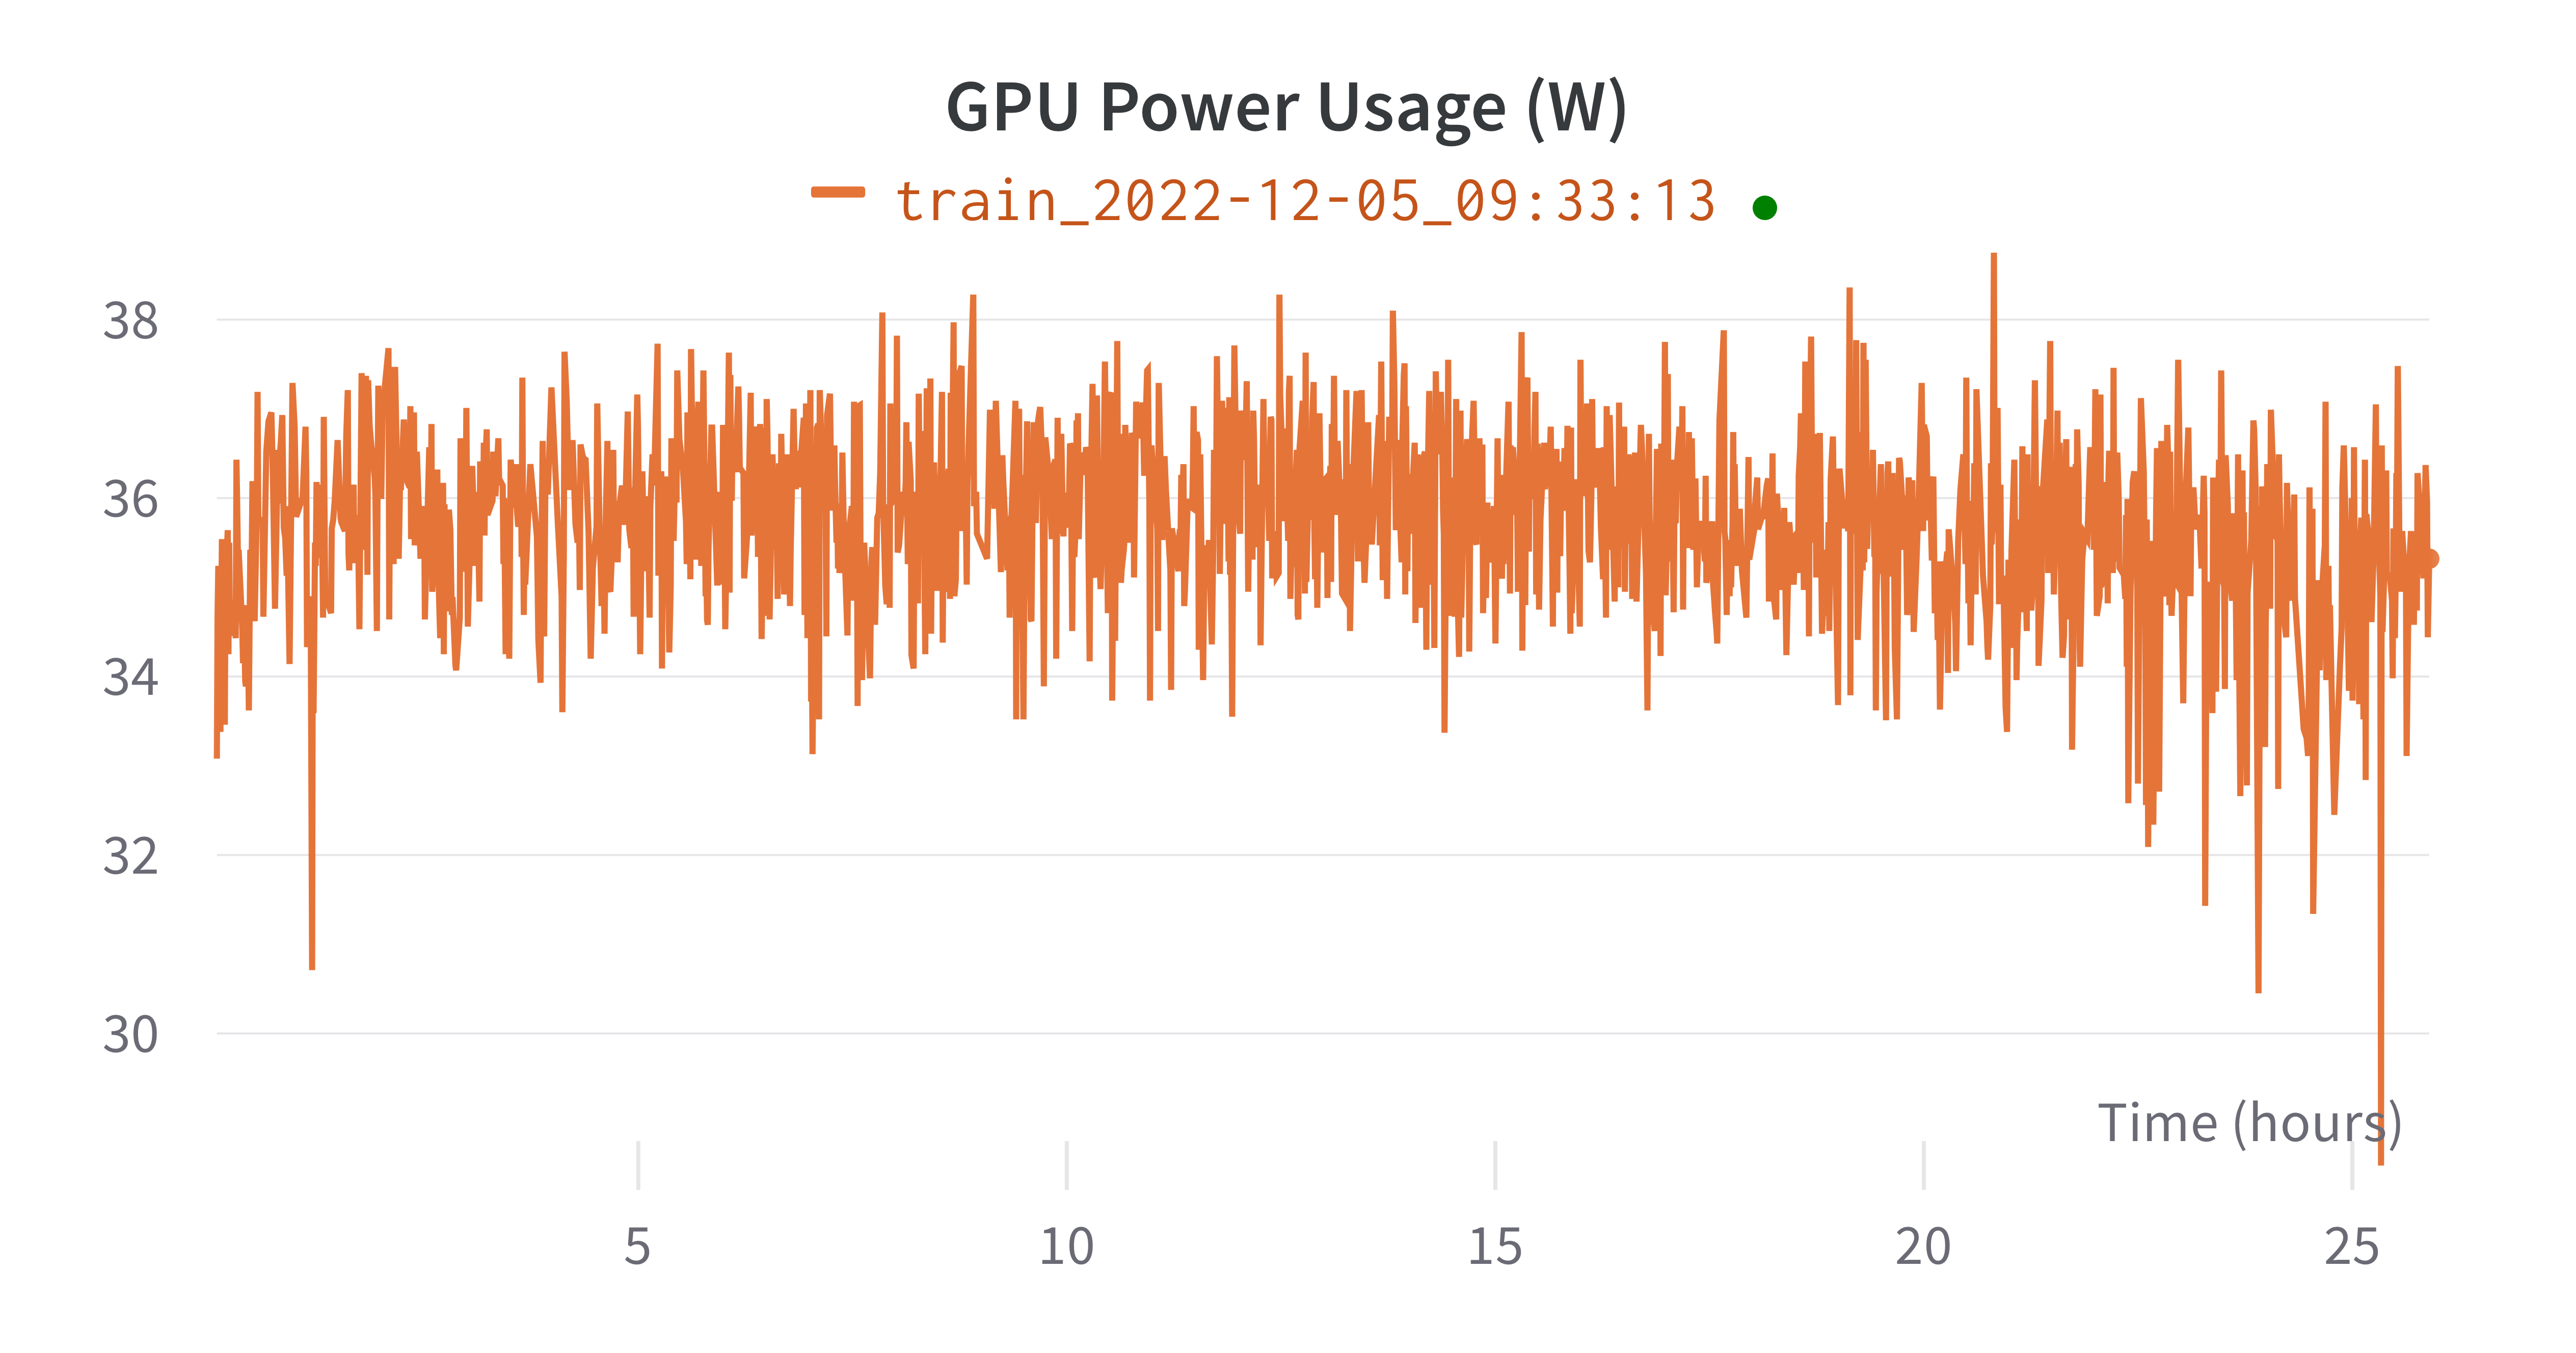
\includegraphics[height=0.25\textwidth]{powerGPU} \label{fig:gpu-pow1}}
			\subfigure{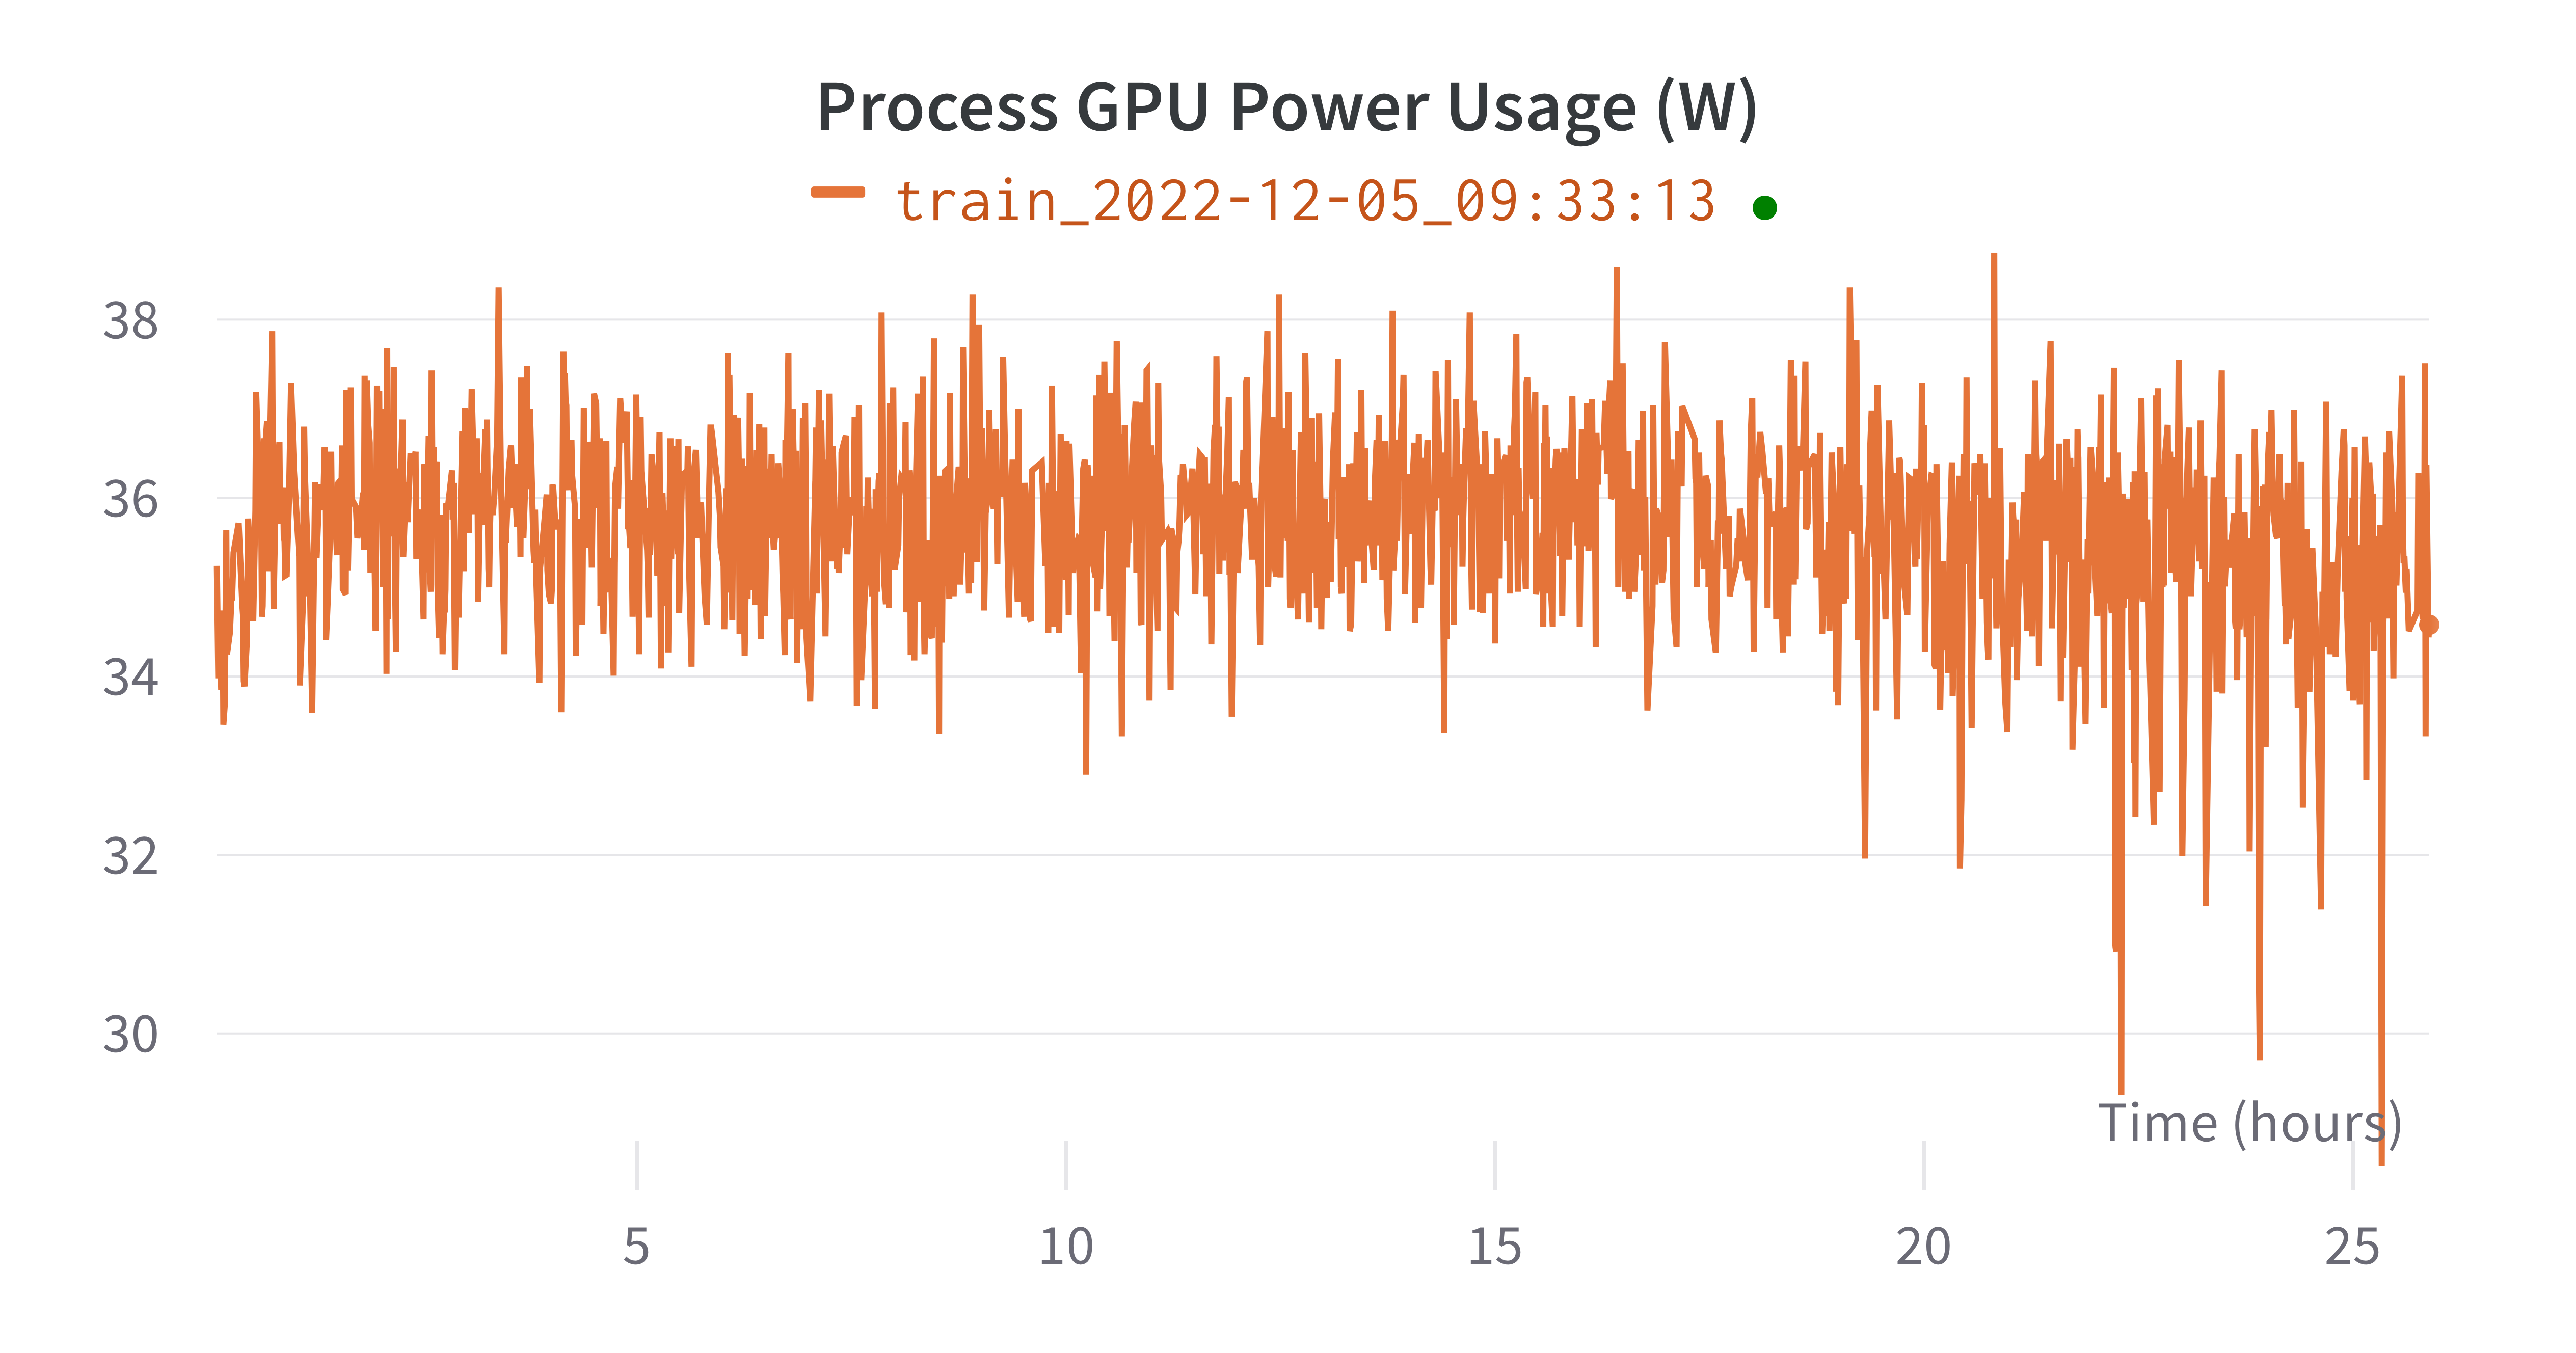
\includegraphics[height=0.25\textwidth]{processGPUPower} \label{fig:gpu-pow2}}
		\caption{Power consumption of GPU.}
	\end{figure}
		
The power consumption (figure~\ref{fig:gpu-pow1}-\ref{fig:gpu-pow2}) of the Graphical Processing Unit appears to be approximately 35Wh.

	\begin{figure}[H]
	{\centering
	  {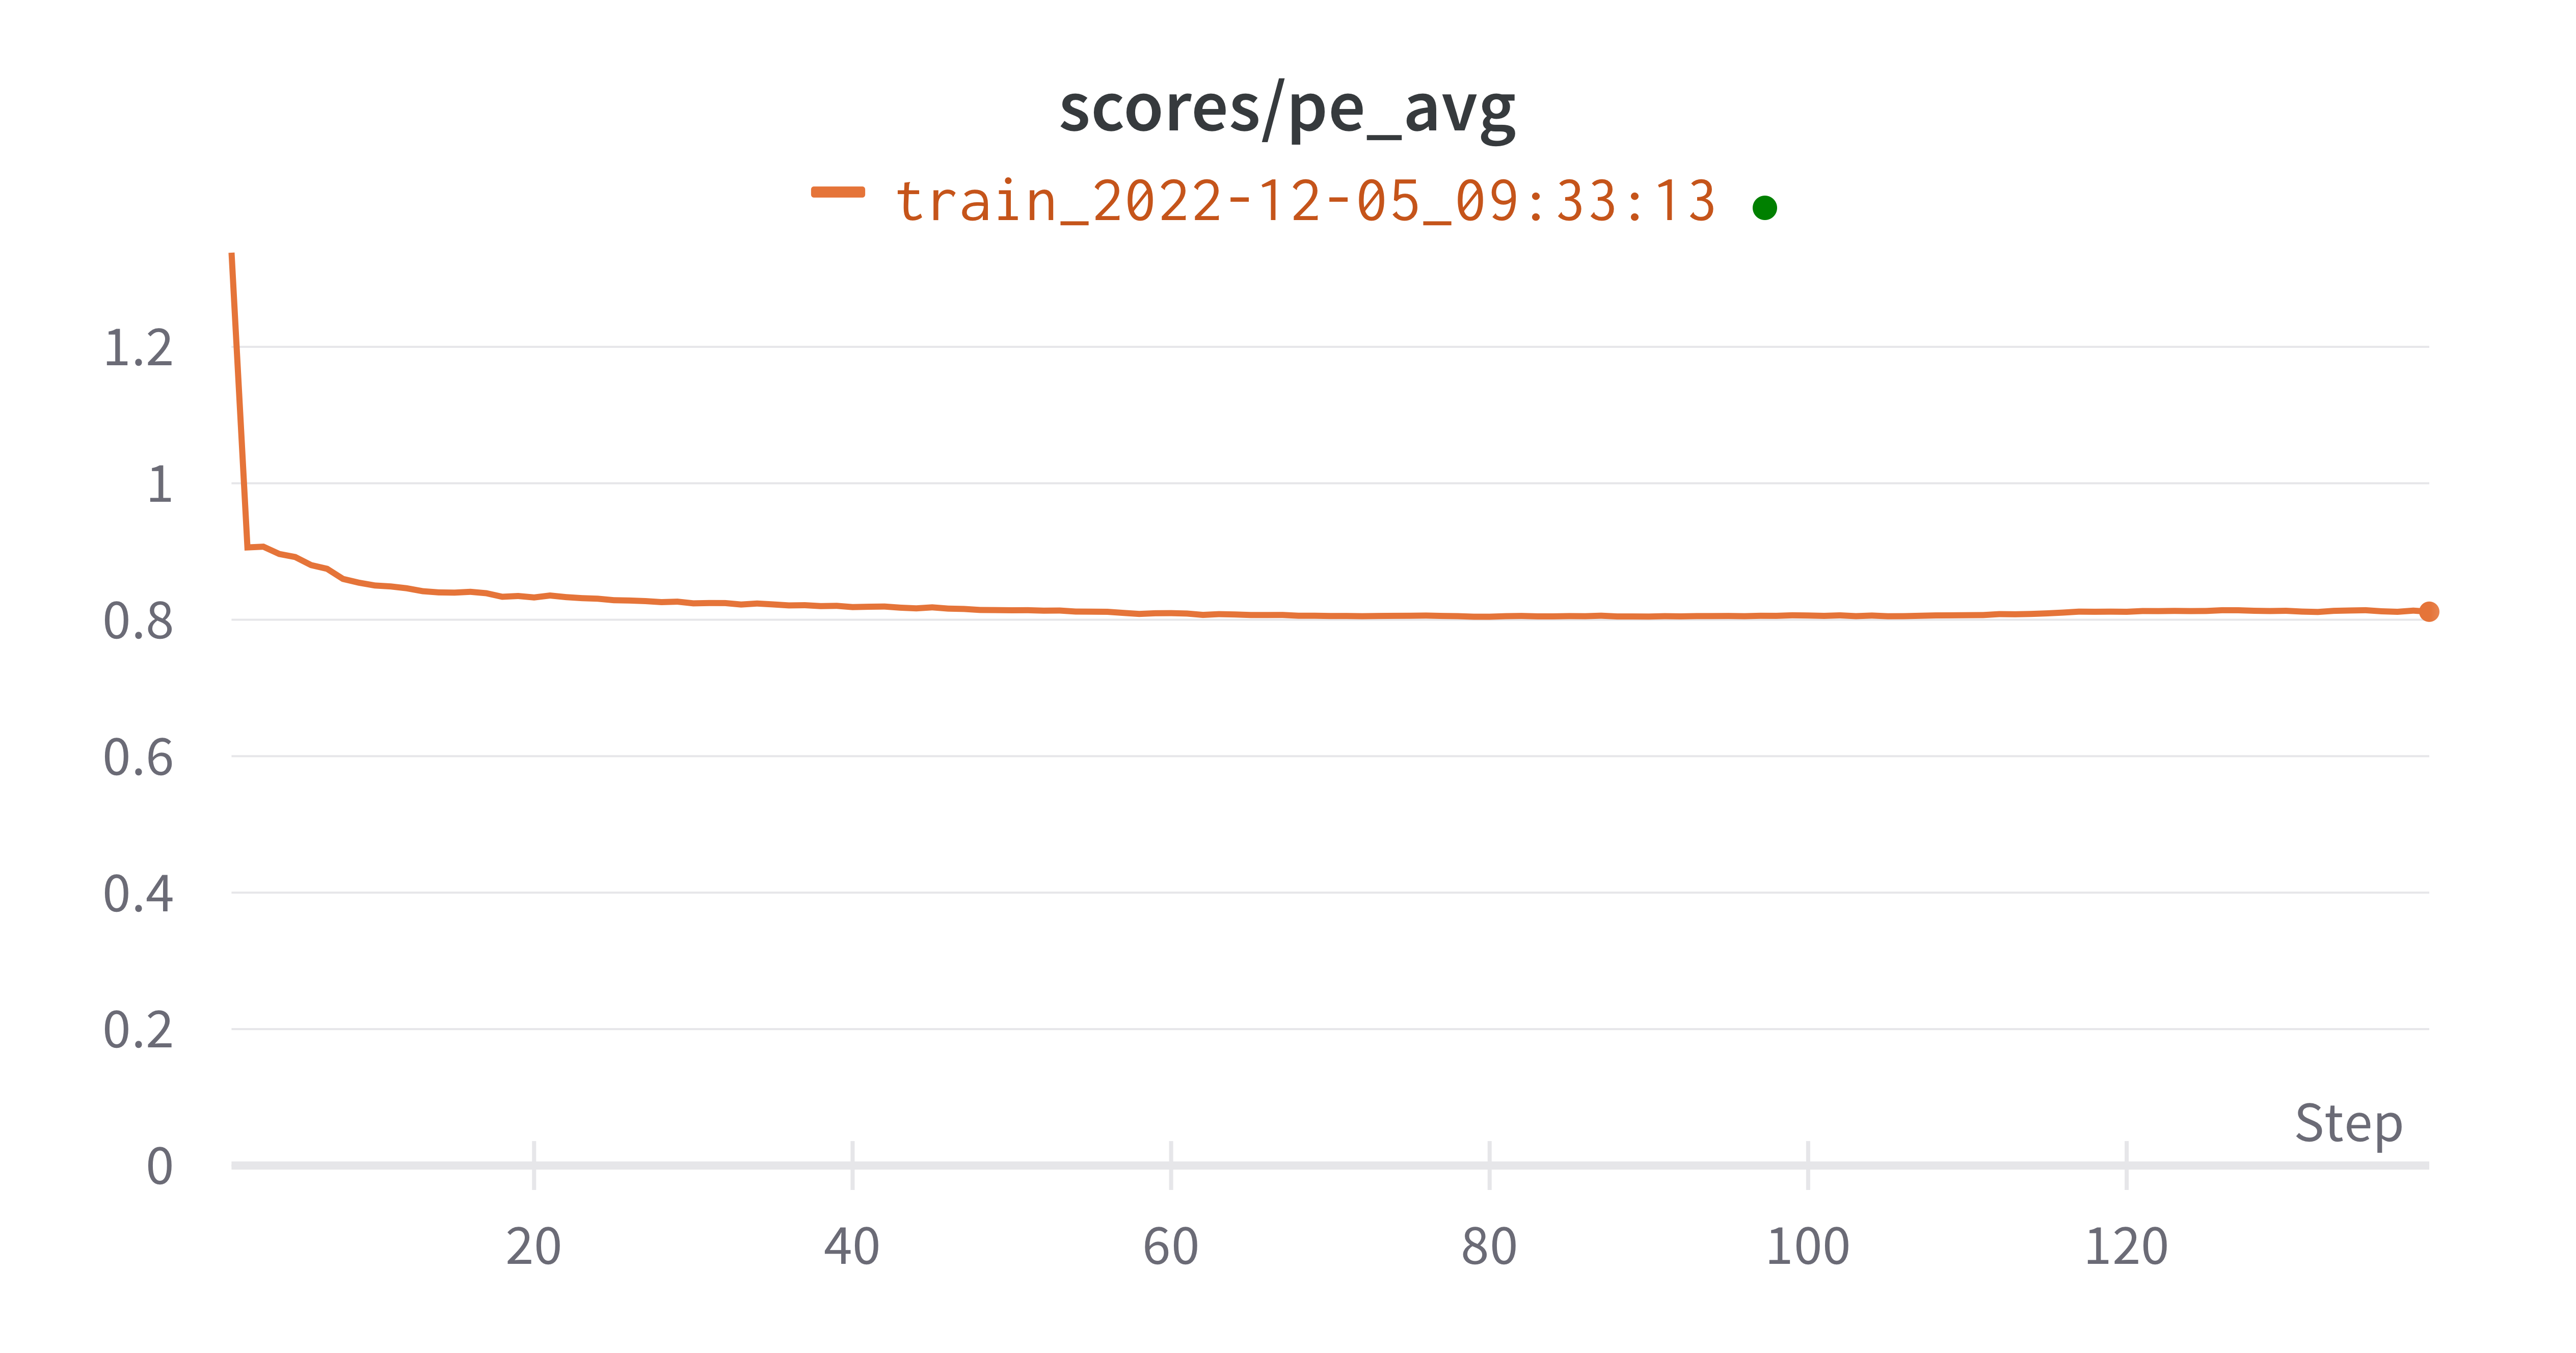
\includegraphics[width = 0.9\textwidth]{peAvgGPU}
	  }
	  \par}
	\caption{Average of Price cost and Emission cost .}
	\label{fig:pe-avg}
	\end{figure}
	
	\begin{figure}[H]
		\centering	
			\subfigure[Price cost]{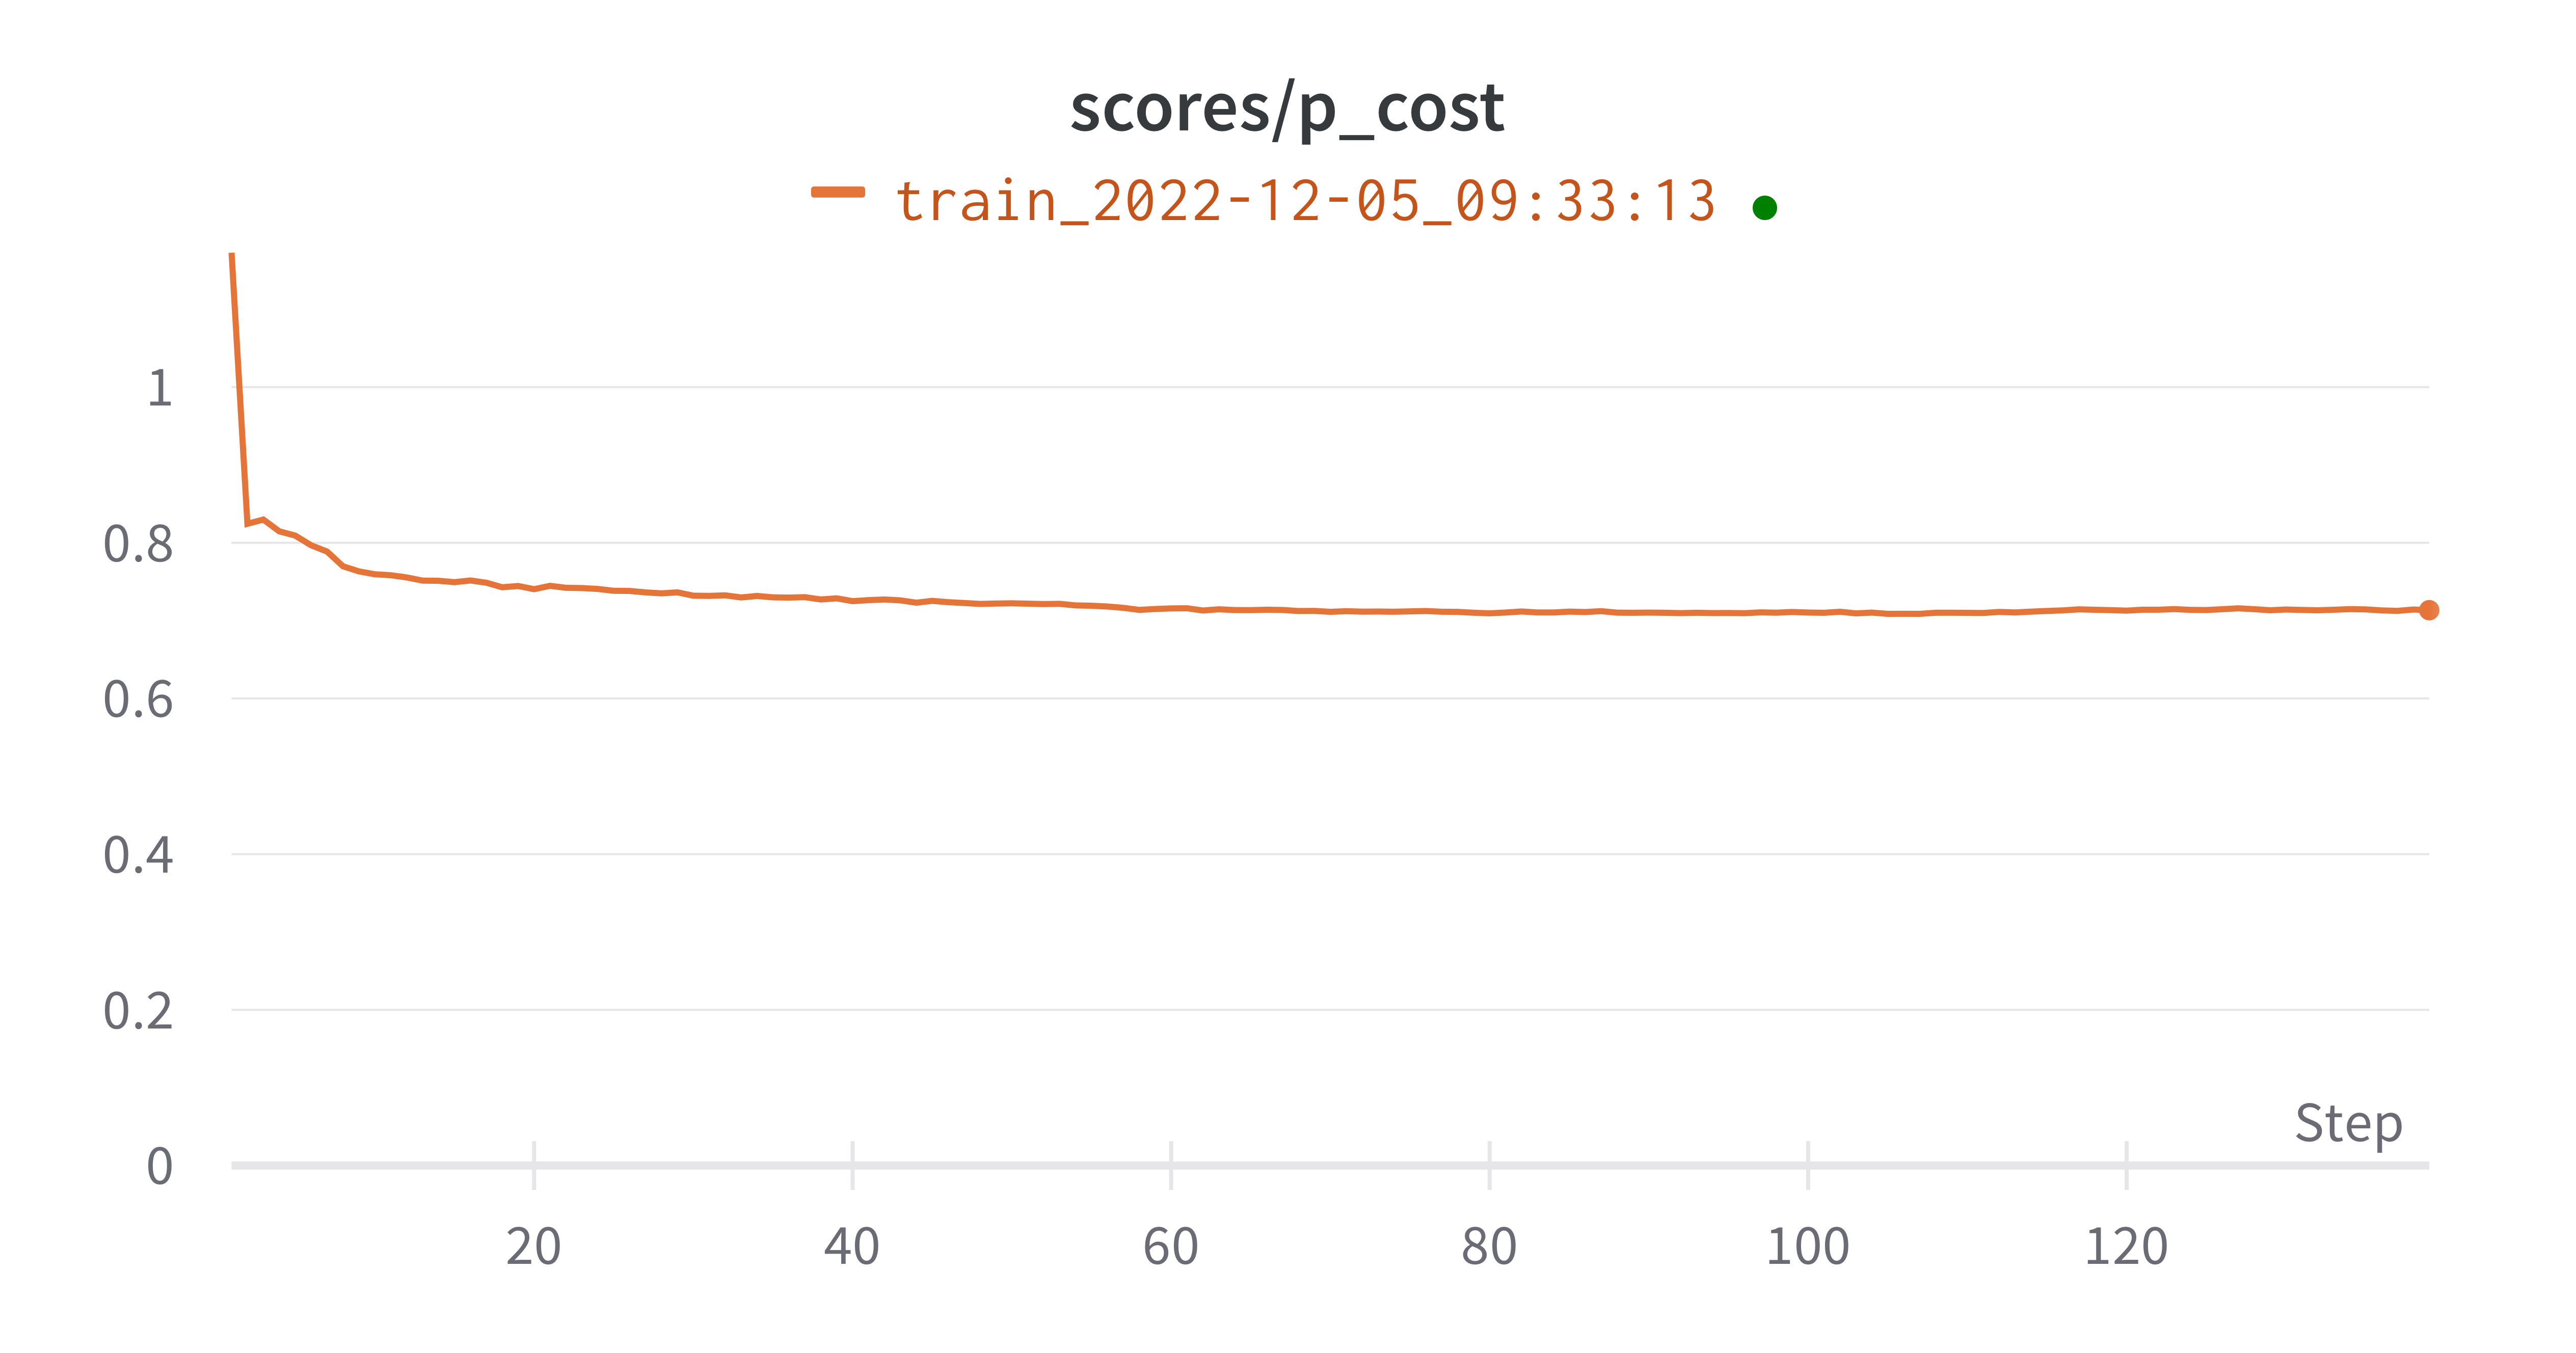
\includegraphics[height=0.25\textwidth]{pCostGPU} \label{fig:p-cost}}
			\subfigure[Emission cost]{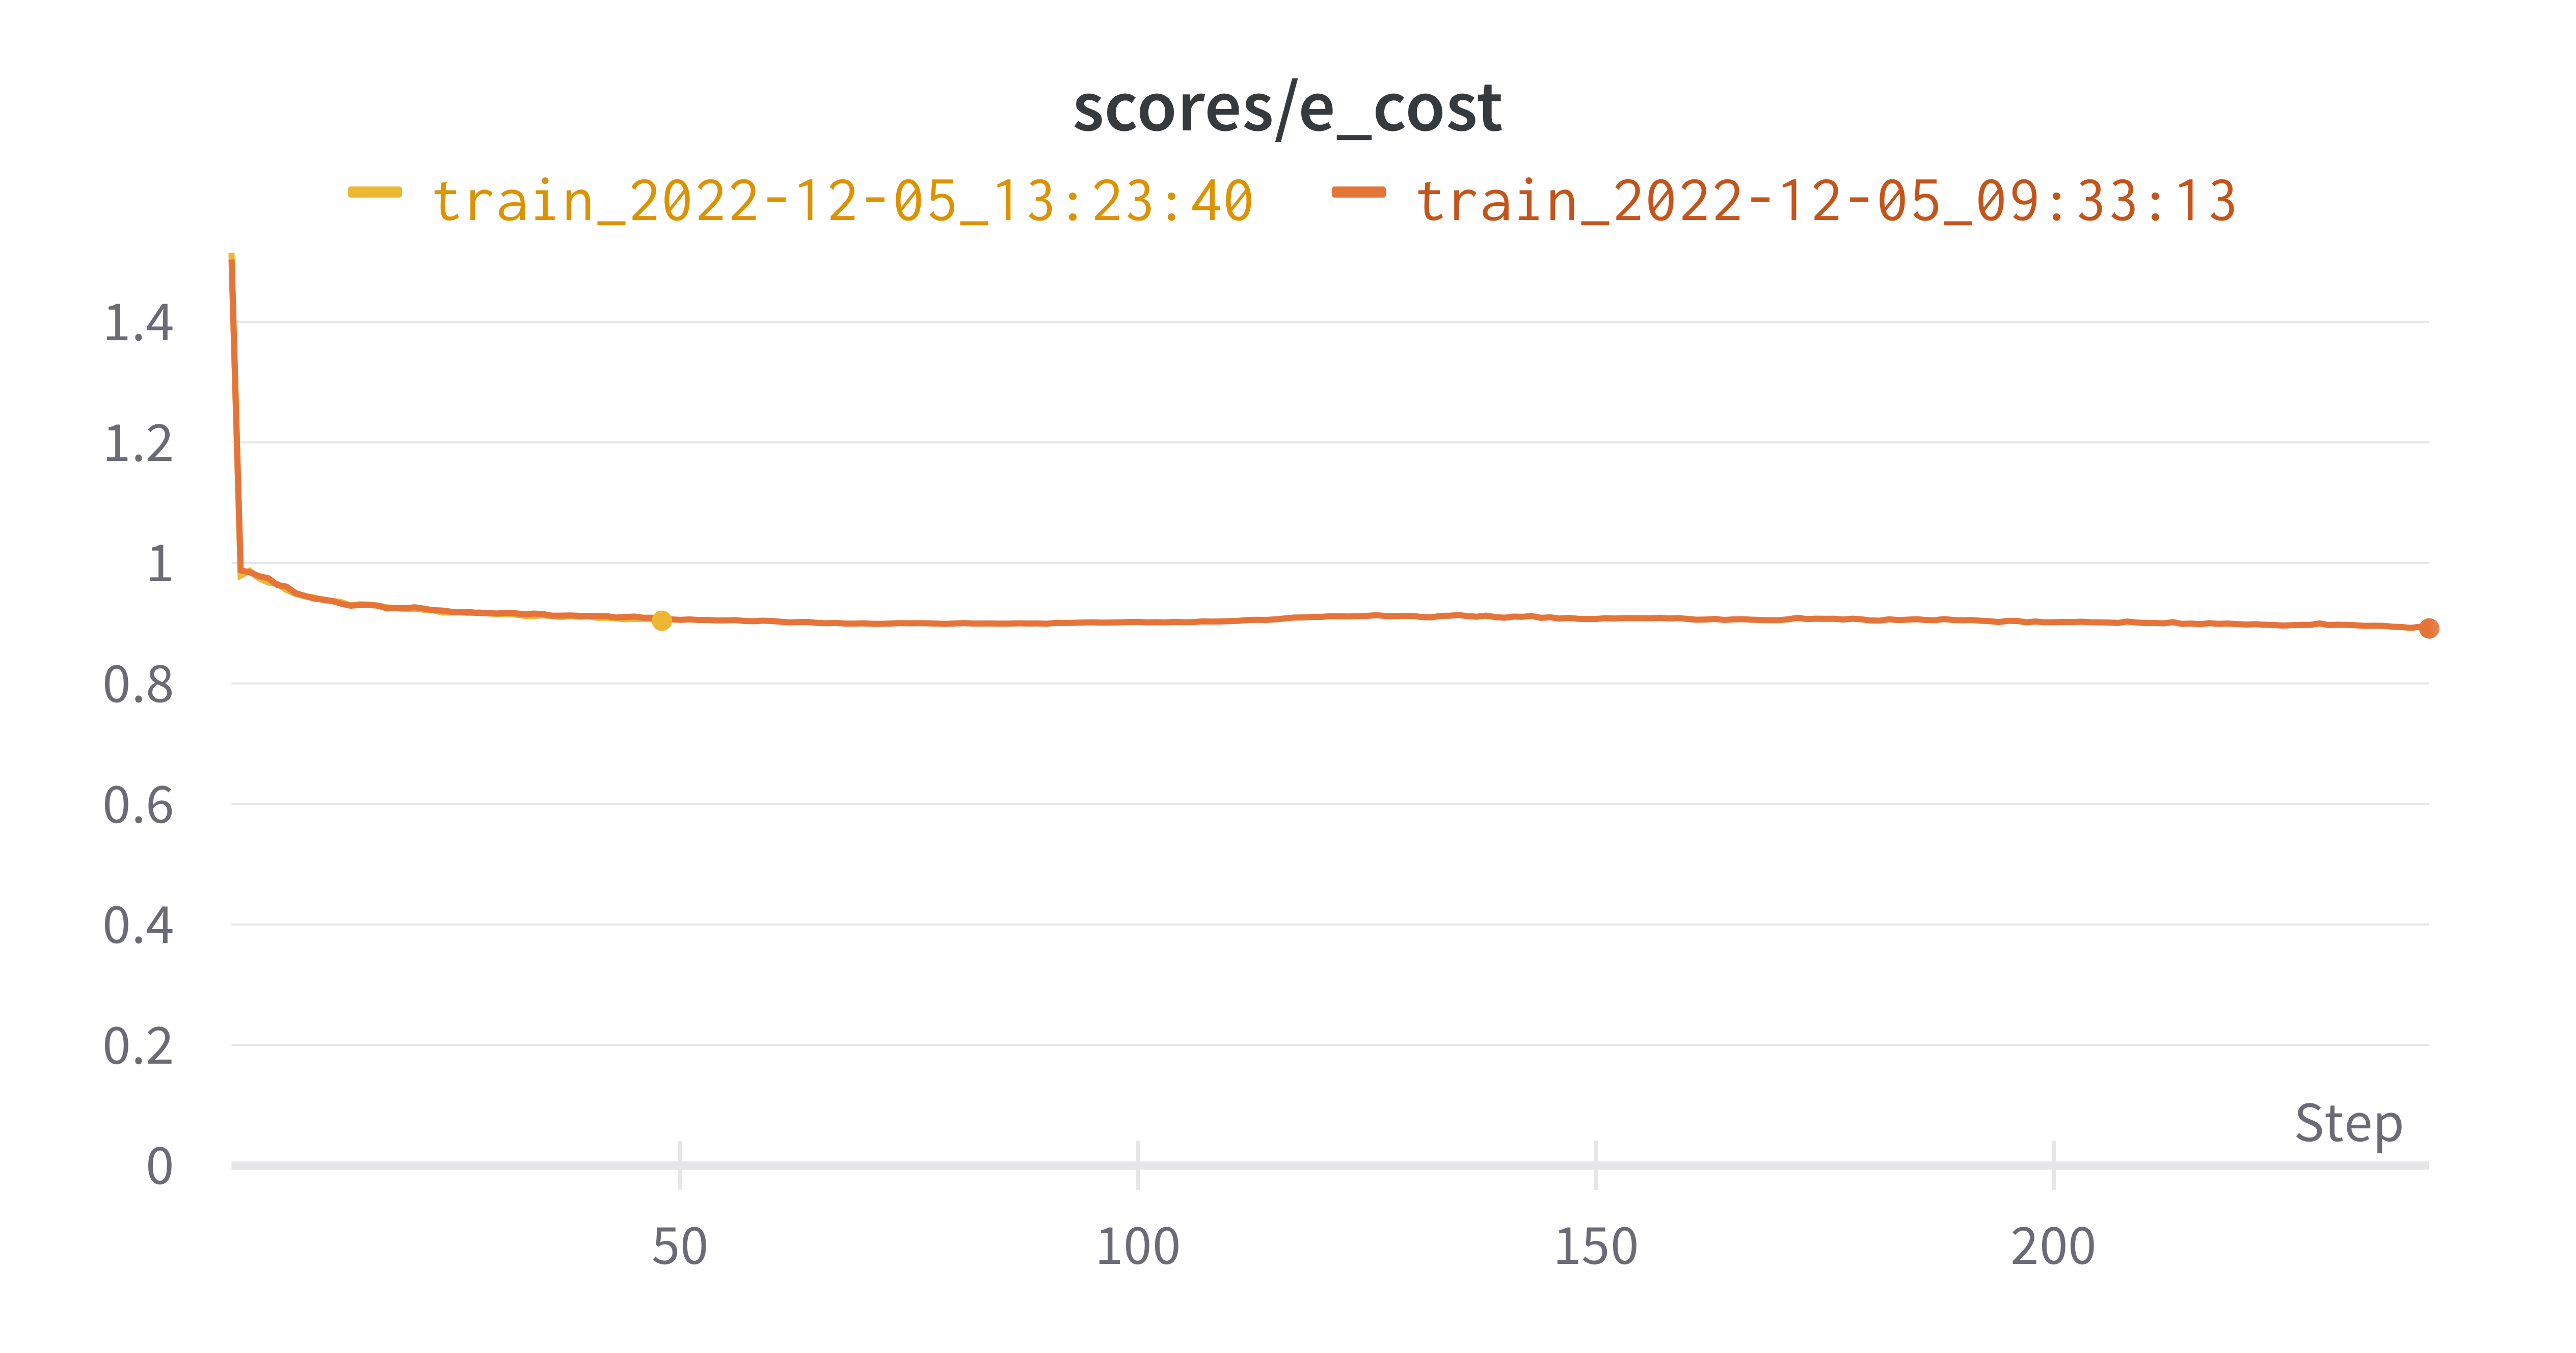
\includegraphics[height=0.25\textwidth]{eCostGPU} \label{fig:e-cost}}
		\caption{Individual target variables.}
	\end{figure}
	
The target variables appear to converge within 250 episodes in around 26 hours resulting in the average of \verb!0.7963! (figure~\ref{fig:pe-avg}) with \verb!0.7013, 0.8912! of Price~\ref{fig:p-cost} and Emission~\ref{fig:e-cost} costs shown in figures. The computation of the last 100 episodes did almost zero change to the results. Running the script on a PC killed the machine after 50 episodes. The cluster run finished successfully. 

The sharp peak at the first iteration is due to the SAC algorithm performing random actions at the beginning to explore the environment and build its policy. 

To conclude Reinforcement Learning with a Soft Actor-Critic approach does look to be interesting and promising, however, training takes a large amount of time and energy even given a small dataset (5 sets of 12 variables with 8000 values each). 


%\newpage
		

\bibliographystyle{plain}
\bibliography{refs.bib}
			 	
	 	
	 	


 


\end{document}